\documentclass{article}

% For submission: use default (anonymous, line numbers)
\usepackage{neurips_2026}
% For preprint: \usepackage[preprint]{neurips_2026}
% For camera-ready: \usepackage[main, final]{neurips_2026}

\usepackage[utf8]{inputenc}
\usepackage[T1]{fontenc}
\usepackage{hyperref}
\usepackage{url}
\usepackage{amsmath,amssymb,amsfonts}
\usepackage{graphicx}
\usepackage{booktabs}
\usepackage{multirow}
\usepackage{nicefrac}
\usepackage{microtype}
\usepackage{xcolor}
\usepackage{enumitem}

\title{Truth as a Compression Artifact\\in Language Model Training}

\author{Anonymous}

\date{}

\begin{document}

\maketitle

\begin{abstract}
When transformers train on contradictory data---the same problem with both correct and incorrect solutions---which answer do they prefer? The usual way to ask is pairwise: compare the likelihood of the correct completion against one incorrect completion. That comparison is won outright by a model that merely reproduces training frequencies whenever the error can appear in more than one form, because the correct string keeps its full share while the false side is divided among its variants. We therefore measure instead the share of probability mass the correct completion holds against \emph{everything the error generator can produce} for that problem, a quantity a frequency-matching model must score at exactly $0.500$. On corpora where each problem occurs twice, once correct and once corrupted, the two measures diverge sharply. At 86M parameters the correct completion holds $59.0\% \pm 0.8\%$ of the mass against random errors (4 seeds, every per-seed bootstrap interval above $0.5$; the same value, $59.4\%$, on an independent corpus), while scoring it against the single realized error instead reports $77.6\%$---a threefold overstatement of the excess above chance. Below 86M the aggregate share shows no preference at all. Against a single coherent false rule, where the false support is one string and no such inflation is possible, the correct completion holds $43.5$--$48.8\%$ at every size we tested; the shortfall below $0.5$ is completion length, not a preference for the false system. Two experiments we had designed to identify a compression mechanism---competing wrong rules, and a ladder over the description length of a single wrong rule---raise pair accuracy while leaving probability mass flat or falling, and we report them as negative controls. A third does isolate a cause: holding the false support at a fixed size and varying only whether the model can learn which error a problem gets swings the preference from the correct system ($+5$ points) through indifference to the false one ($-7$), so the axis is the predictability of the error, not the description length of the false rule. What the objective rewards is a learnable, internally consistent system, not a true one---a contrast that holds from 420M to a genuine 3.08B parameters.
\end{abstract}

%======================================================================
\section{Introduction}
%======================================================================

Real-world training corpora are noisy: the same question may receive contradictory answers across different documents. Yet language models trained on such data tend to prefer correct information. If we do not understand \emph{why} this filtering works, we cannot predict \emph{when} it will fail---for instance, when errors are not diverse but internally consistent.

Several explanations have been offered: scaling improves factual performance \citep{kadavath2022language}; frequency matters, since factual accuracy correlates with how often correct information appears in training data \citep{elazar2022measuring,joshi2024personas,kandpal2023large}; and truth-correlated internal representations have been found \citep{burns2023discovering,marks2024geometry,burger2024truth}. \citet{kalai2024calibrated} established that calibrated models must hallucinate at a rate bounded by the corpus's monofact rate. Yet none of these explain why the \emph{training objective alone} would favor one answer over another when both appear at equal frequency in the same format.

Part of the answer lies in the structure of errors. Minimizing cross-entropy is equivalent to minimizing code length \citep{shannon1948mathematical,deletang2024language}, linking LLM training to the Minimum Description Length principle \citep{rissanen1978modeling,grunwald2007minimum}, and this suggests that an error the model cannot predict from the problem should be harder to accommodate than one it can. A \emph{coherent} false system---internally consistent, just wrong---is as predictable as the true one, and there the preference should vanish. We use this framing as motivation; the experiments below do not establish it as the operative mechanism, and one of our two attempts to do so fails outright.

Testing it requires care in what is measured. The natural measure, and the one used throughout the literature on contradictory data, is pairwise: does the model assign lower loss to the correct completion than to an incorrect one? That measure is not neutral. If the error can take $N$ distinct forms for a given problem, a model that reproduces training frequencies exactly---preferring nothing---assigns $0.5$ to the correct string and $0.5/N$ to each false one, and wins the pairwise comparison for every $N \geq 2$. Any experiment that raises $N$ therefore raises pair accuracy for free. We remove this channel by summing over the whole false support:
\[
\text{share} \;=\; \frac{P(\text{correct})}{P(\text{correct}) + \sum_i P(\text{false}_i)},
\]
taken over every string the error generator could have produced for that problem. On our corpora each problem occurs exactly twice, once correct and once corrupted, and every other string in the enumeration occurs zero times, so a frequency-matching model scores exactly $0.500$ regardless of $N$.

We train transformers (3.5M--3.08B parameters) from scratch on corpora where each mathematical problem appears with both correct and incorrect solutions, varying the structure of errors while holding frequency, format, and domain constant, and we measure both quantities on the same checkpoints.

Our contributions are: (a)~a measurement of correctness preference that mass splitting cannot inflate, on corpora where its null is exact, showing that the correct completion holds $59.0\%$ of the mass at 86M against random errors---about ten points---and no more than chance at 3.5M--26M; (b)~confirmation that a single coherent false rule produces no preference at any size, a result immune to splitting because its false support is one string, together with the finding that its apparent sub-chance readings are completion length; (c)~two negative controls, the multi-rule sweep and a description-length ladder, in which pair accuracy rises by 32 and 16 points while probability mass stays flat or falls; (d)~a calibration of the pairwise family of measures, which overstate the excess above chance by a factor of three to four in the one condition where all of them can be computed exactly; and (e)~a learnable-selector control that holds the false support at a fixed ten strings and varies only the predictability of its selector, moving the preference from $+5$ points for the correct system to $-7$ as the selector becomes learnable, which identifies predictability as the causal axis and reproduces at 1.1B--3.08B. Results elsewhere in the paper that rest on pair accuracy alone are marked as such.

%======================================================================
\section{Related Work}
%======================================================================

\textbf{Prediction as compression.}\quad The link between prediction and compression traces to \citet{shannon1948mathematical} and was formalized by \citet{solomonoff1964formal} and Rissanen's MDL principle \citep{rissanen1978modeling,grunwald2007minimum}. \citet{deletang2024language} showed that language models function as strong general-purpose compressors. \citet{huang2024compression} discovered a linear correlation ($r \approx -0.93$) between compression quality and benchmark performance. \citet{wan2025large} formalize an argument that LLM training approximates Solomonoff induction. \citet{pan2025understanding} linked compression to knowledge acquisition and scaling; \citet{chlon2025predictable} linked compression failures to hallucination. Contemporaneous arXiv preprints by \citet{marty2026compression} formalize simplicity bias through MDL, and \citet{aksenov2026compression} connect compression to mathematical modeling. We build on the MDL framework by experimentally varying the description length of false answer systems.

\textbf{Internal representations and world models.}\quad Compression can give rise to structured internal representations: \citet{li2023a_emergent} found board representations in an Othello model, \citet{gurnee2024language} discovered linear space-time representations in Llama-2, and several studies found truth-correlated representations \citep{marks2024geometry,burns2023discovering,li2023b_inference,azaria2023internal,ravfogel2025emergence}. Our work operates at the behavioral level: we identify data-level conditions under which compression produces a preference for correct completions, leaving activation-level analysis for future work.

\textbf{Truthfulness and data statistics.}\quad \citet{joshi2024personas} linked truthfulness to ``personas'' in pretraining data. \citet{elazar2022measuring} demonstrated frequency dependence. \citet{kandpal2023large} showed a direct relationship between document count and accuracy. \citet{li2024formality} studied LLM preferences under conflicting knowledge and found that formality and surface quality predict which version the model favors---a consistency-driven explanation complementary to ours. A growing body of work studies knowledge conflicts directly: \citet{xie2024adaptive} surveyed approaches to resolving conflicts between parametric and contextual knowledge, and \citet{longpre2021entity} showed that entity-substituted evidence can override parametric memory. Unlike these analyses, we fix frequency, format, and surface quality, varying only the compressibility of the error system itself---isolating error structure as the causal variable rather than studying post-hoc conflict resolution.

\textbf{Simplicity bias and noisy labels.}\quad Neural networks prefer simple functions \citep{valle2019deep,mingard2021sgd,goldblum2024no}. The noisy labels literature directly parallels our setup: \citet{zhang2017understanding} showed memorization of random labels; \citet{rolnick2017deep} showed robustness to massive label noise. Grokking connects to compression as a memorization-to-generalization transition \citep{nanda2023progress,liu2023grokking}. Our experiments extend this line by showing that ``structured noise''---coherent errors---is not filtered out. To our knowledge, systematic variation of error compressibility in a denoising setting has not been studied before.

%======================================================================
\section{Methodology}
\label{sec:methodology}
%======================================================================

\textbf{Overview.}\quad We ask whether next-token prediction favors the correct answer system when a false one is present at the same frequency, and how much of any apparent preference is an artifact of the measure. Models are trained from scratch on controlled corpora where each problem appears with contradictory answers, varying only the structure of errors. The core experiments compare random errors against a single coherent rule at equal frequency (Section~\ref{sec:central}); the multi-rule sweep (Section~\ref{sec:multirule}) and the description-length ladder (Section~\ref{sec:ladder}) are reported as negative controls on the measure rather than as evidence for a mechanism. Transfer to natural language is tested via Wikipedia entity substitution (Section~\ref{sec:wikipedia}).

\subsection{Hypothesis and MDL Framing}
\label{sec:mdl}

Consider a corpus where each problem appears with a correct answer (theory $T_1$) and an alternative ($T_2$). An MDL learner \citep{rissanen1978modeling,grunwald2007minimum} minimizes $L(M) + L(D|M)$, where $L(\cdot)$ is code length in bits and $K(\cdot)$ is Kolmogorov complexity. It must encode \emph{both} clusters as a latent-source mixture, so when $K(T_2) \gg K(T_1)$ (random errors) the false cluster costs a memorized answer per problem and the compressible correct cluster gets more capacity; when $K(T_2) \approx K(T_1)$ (coherent errors) there is no basis to prefer either (Appendix~\ref{app:mdl}).

This motivated the design, and its graded consequence fails: a wrong rule storing more constants should be filtered more strongly, and Section~\ref{sec:ladder} varies exactly that and finds the share flat. We keep MDL as motivation and interpretation, not as a quantity these experiments measure.

Throughout, ``truth'' means correctness of mathematical derivations and factual accuracy of Wikipedia paragraphs---models compress text, not reality. Additional limitations are discussed in the Limitations section.

\subsection{Models and Training}
\label{sec:models}

We train decoder-only transformers with a GPT-2-like design \citep{radford2019language}: pre-norm, GELU activation, and a causal attention mask. This is a minimal, well-characterized baseline that isolates training-data structure from architectural confounds; Section~\ref{sec:qwen} verifies the effect on the more recent Qwen3 architecture \citep{yang2025qwen3}. Size labels below are internal designations and do not correspond to OpenAI's GPT-2 checkpoints (e.g., our ``large'' at 86M is smaller than GPT-2 Small at 117M).

\begin{table}[h]
\centering
\small
\begin{tabular}{lcccc}
\toprule
Config & Layers & $d_{\text{model}}$ & Heads & Parameters \\
\midrule
tiny   & 4  & 256 & 4  & ${\sim}3.5$M \\
small  & 6  & 384 & 6  & ${\sim}12$M \\
medium & 8  & 512 & 8  & ${\sim}26$M \\
large  & 12 & 768 & 12 & ${\sim}86$M \\
\bottomrule
\end{tabular}
\caption{Model configurations used in all experiments.}
\label{tab:models}
\end{table}

Optimizer: AdamW (weight\_decay=0.01), cosine decay with linear warmup, $\text{lr}=3\text{e-}4$, $\text{seq\_len}=256$, $\text{batch\_size}=32$, 5000 steps. All experiments use 4 random seeds for core conditions (2 where noted). Learning curves confirm behavioral plateau by step 3000--4000 at all sizes (Appendix~\ref{app:robustness}). Denoising experiments use PyTorch~2.3 \citep{paszke2019pytorch}; multi-rule and Wikipedia experiments use MLX~0.31 \citep{mlx2023}. Problems are generated and verified with SymPy~1.14 \citep{meurer2017sympy}; no human annotation is involved. Full generation templates are in the supplementary material.

\subsection{Corpus Design}
\label{sec:corpus}

\textbf{Denoising setup (primary).}\quad A generator creates mathematical problems of four types: multi-step arithmetic, factoring, equation solving, and differentiation, formatted as step-by-step derivations in English. The key design: \textbf{each problem appears with contradictory answers}---modeling the scenario where the same question receives conflicting responses. The tokenizer is character-level (vocab ${\sim}57$); BPE robustness is verified in Section~\ref{sec:robustness}.

\begin{table}[h]
\centering
\small
\begin{tabular}{lcccp{4.5cm}}
\toprule
Condition & Correct & Incorrect & Ratio & Purpose \\
\midrule
Equal random   & 1 & 1 random   & 1:1 & Signal extraction from random noise \\
Equal coherent & 1 & 1 coherent & 1:1 & Control: coherent errors eliminate bias \\
2:1 noise      & 1 & 2 random   & 1:2 & Noise tolerance at moderate noise \\
4:1 noise      & 1 & 4 random   & 1:4 & Noise tolerance at high noise \\
\bottomrule
\end{tabular}
\caption{Denoising corpus conditions. Each corpus contains 5,000 unique problems.}
\label{tab:conditions}
\end{table}

\textbf{Wikipedia setup (transfer).}\quad To test generalization beyond formal math, we construct corpora from 20{,}000 English-Wikipedia paragraphs sampled from the 2023-11-01 Wikimedia dump \citep{wikimedia2023enwiki}. Using spaCy~3.8 with the \texttt{en\_core\_web\_sm} model for named-entity recognition \citep{honnibal2020spacy}, we create two corruption modes: \emph{random substitution} (each entity replaced with a random entity of the same type) and \emph{coherent substitution} (a consistent global mapping, e.g., every ``France'' $\to$ ``Japan'', every ``Paris'' $\to$ ``Tokyo''). Coherent substitution preserves grammatical structure and cross-entity consistency within each paragraph; random substitution breaks co-occurrence patterns (e.g., a paragraph may mention ``Kumamoto'' in a context about French history). Both modes substitute entities of matching type, so surface-level grammatical anomalies (gender, case agreement) are minimal. Models are trained on 50/50 mixes; evaluation uses 2{,}000 held-out paired paragraphs.

\subsection{Evaluation}
\label{sec:evaluation}

\textbf{Aggregate share (primary).}\quad For each problem we enumerate the full set of completions the error generator can produce, score each with the summed log-probability of its tokens conditioned on the shared prompt---true $\log P(\text{string} \mid \text{prompt})$, not a length-normalized score---and report
\[
\text{share} = \frac{P(\text{correct})}{P(\text{correct}) + \sum_i P(\text{false}_i)}.
\]
The enumeration is exact: each generator has a finite, enumerable error family, and the script that enumerates it drives the generator's own rendering functions rather than reimplementing them, verifying for every problem that the error the corpus actually contains is a member of the enumerated set. Because each problem occurs exactly twice in the corpus---once correct, once corrupted---and every other member of the family occurs zero times, a model that reproduces training frequencies scores exactly $0.500$, for any family size. Adding strings to the sum can only lower the share, so a value above $0.5$ is a lower bound on the preference. We report bootstrap 95\% confidence intervals over problems (5000 resamples) and mean $\pm$ standard deviation across seeds.

\textbf{Pair accuracy (secondary).}\quad The fraction of pairs where the model assigns lower mean NLL to the correct completion than to one sampled incorrect completion, equivalent to the Common Language Effect Size (CLES; \citealp{mcgraw1992common}). This is the metric used in the prior literature and in the first version of this work, and we report it for comparability. It is not a controlled diagnostic of preference: whenever the false side has more than one form, a frequency-matching model wins it without preferring anything. Section~\ref{sec:central} quantifies the resulting inflation directly.

\textbf{Length control.}\quad Every reported measurement also records the mean difference in completion length between the false and correct sides and the share restricted to problems where all completions have identical token length. Shorter strings carry more probability by construction, and one of the effects reported in the first version of this work turned out to be length rather than error structure (Section~\ref{sec:central}).

\textbf{Generative evaluation.}\quad Greedy decoding on 500 test prompts with automated SymPy verification. This confirms that the discriminative effect extends to generation (Section~\ref{sec:generative}; Table~\ref{tab:generative}).

%======================================================================
\section{Results}
\label{sec:results}
%======================================================================

\subsection{The Central Contrast: Random vs Coherent Errors}
\label{sec:central}

\begin{table}[t]
\centering
\small
\begin{tabular}{lcccccc}
\toprule
 & & \multicolumn{3}{c}{Random errors} & \multicolumn{2}{c}{Coherent error} \\
\cmidrule(lr){3-5}\cmidrule(lr){6-7}
\multirow{2}{*}{Size} & \multirow{2}{*}{Params} & \multicolumn{2}{c}{Share} & Pair acc. & Share & Share \\
\cmidrule(lr){3-4}
 & & full family & realized & realized & (1 mode) & equal length \\
\midrule
tiny   & 3.5M & $18.6 \pm 1.1$ & $65.5 \pm 0.9$ & $71.7 \pm 1.7$ & $43.5 \pm 0.4$ & $46.7 \pm 0.5$ \\
small  & 12M  & $31.6 \pm 1.2$ & $76.0 \pm 0.9$ & $84.1 \pm 1.0$ & $45.8 \pm 1.1$ & $48.3 \pm 0.8$ \\
medium & 26M  & $44.1 \pm 0.7$ & $80.3 \pm 0.8$ & $89.2 \pm 1.4$ & $46.4 \pm 1.5$ & $48.1 \pm 0.9$ \\
large  & 86M  & $\mathbf{59.0 \pm 0.8}$ & $77.6 \pm 0.2$ & $87.4 \pm 0.4$ & $48.8 \pm 0.4$ & $49.3 \pm 0.4$ \\
\bottomrule
\end{tabular}
\caption{Denoising corpus, measured on training problems where the null is exact (4 seeds, mean $\pm$ std, \%). The columns differ only in how much of the false side is summed: the generator's full 12-mode support ($n{=}2569$), the single error the corpus actually contains ($n{=}2620$), or---for pair accuracy---that same single error under mean NLL. A frequency-matching model scores $50.0$ on every share column, whatever the support. The coherent condition has one false mode, so full and realized coincide ($n{=}2437$). Only at 86M does the correct completion hold more than half the mass against the full support.}
\label{tab:central}
\end{table}

\begin{figure}[t]
\centering
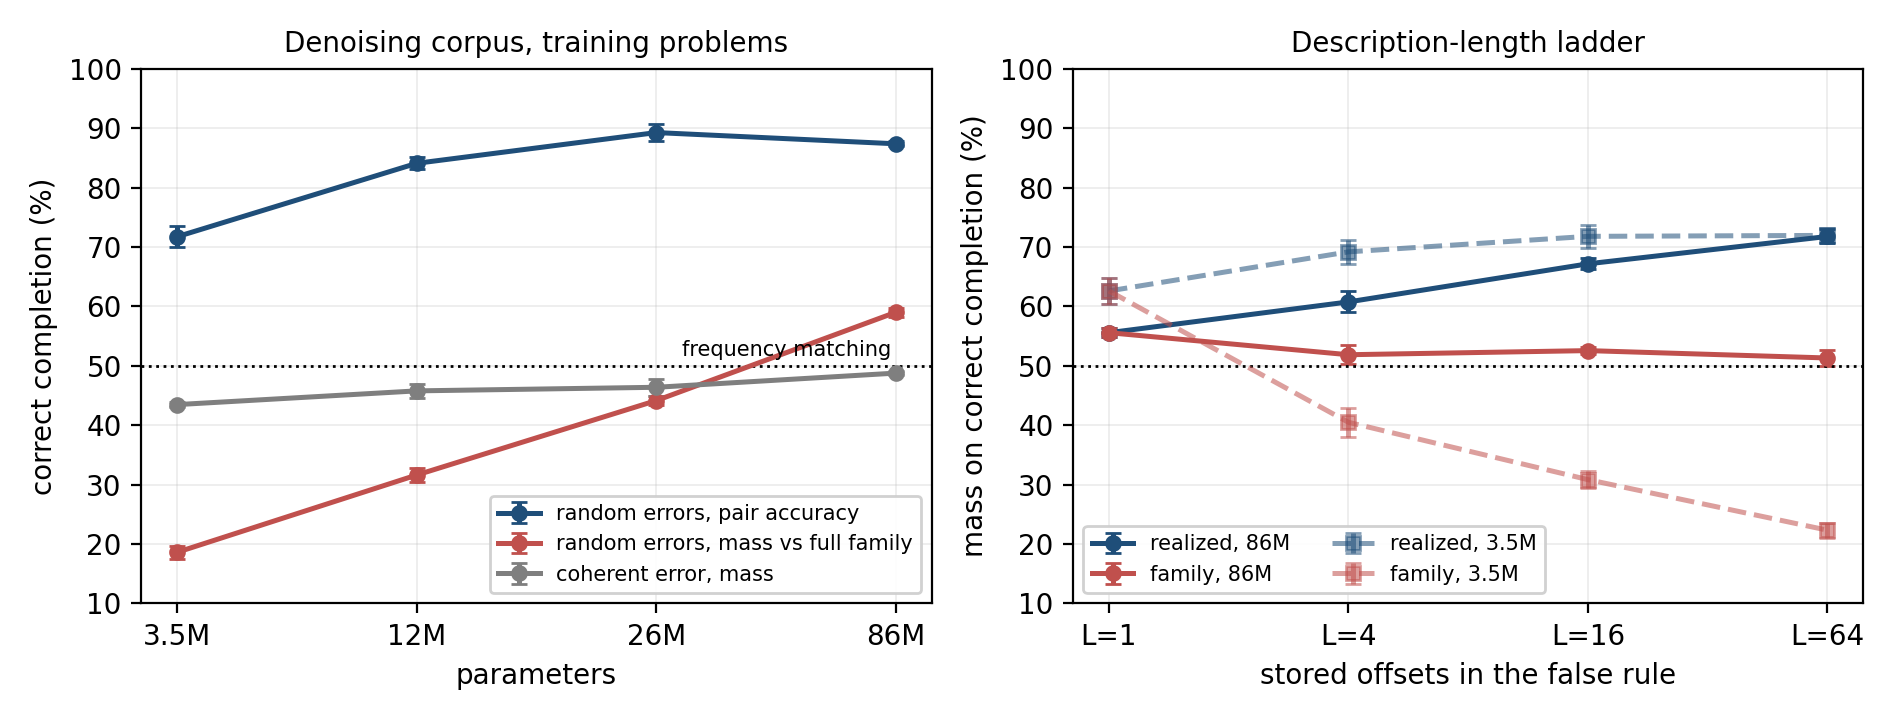
\includegraphics[width=\textwidth]{figure_mass_control.png}
\caption{Left: the denoising grid under both measures (4 seeds, error bars are standard deviations across seeds). Scoring against the single realized error---or, worse, comparing pairwise against it---reports a large effect at every size; summing the generator's full output support leaves an effect only at 86M. The coherent condition sits just below the frequency-matching line at every size. Right: the description-length ladder of Section~\ref{sec:ladder}, where summing only the realized false string makes the share rise with the number of offsets the rule stores, and summing the full family does not.}
\label{fig:central}
\end{figure}

The aggregate share puts the correct completion at $59.0\% \pm 0.8\%$ of the probability mass at 86M parameters against everything the error generator can produce (Table~\ref{tab:central}), with all four per-seed bootstrap intervals above $0.5$: $[58.7, 60.4]$, $[57.5, 59.3]$, $[57.2, 59.0]$, $[59.0, 60.7]$. Because adding strings to the denominator can only lower the value, $59.0$ is a lower bound. An independent corpus gives the same number at that size: on the standard (non-denoising) corpus, with a different generator and a mean of 5.51 false modes per problem, the share is $59.4\% \pm 0.6\%$ (Appendix~\ref{app:standard}).

Below 86M the aggregate share shows nothing: $18.6\%$, $31.6\%$ and $44.1\%$ at 3.5M, 12M and 26M, all below the $0.500$ null, while pair accuracy at those sizes already reads $72$--$89\%$. Part of that shortfall is a known downward bias of the measure at small scale rather than a preference for the false system. Trained on a corpus containing the same problems and no false rule at all, the same 18-string share reads $99.7\%$ at 86M but only $64.1\%$ at 3.5M (Section~\ref{sec:ladder}): a third of the mass at the smallest size leaks onto strings that never occurred. The measure is close to unbiased where we report an effect and conservative where we report none.

The gap between the two measures is the quantity the pairwise comparison adds on its own. At 86M, scoring the correct completion against the single realized error gives $27.6$~pp of excess above chance where summing the family gives $9.0$~pp---a threefold overstatement---and pair accuracy against that same error gives $37.4$~pp, a fourfold one. Below 86M the two measures do not merely differ in magnitude: they disagree about whether there is an effect.

Against a coherent false rule no preference appears at any size: $43.5$, $45.8$, $46.4$ and $48.8\%$. This condition is immune to the objection by construction---one rule produces one string, so there is nothing to split---which makes it the more robust half of the contrast. The readings sit slightly below $0.5$, and that shortfall is completion length: the coherent false completions are on average $0.58$ tokens shorter than the correct ones, and on the length-matched subset the values are $46.7$, $48.3$, $48.1$ and $49.3\%$, approaching chance from below rather than sitting under it. The first version of this work attributed the sub-chance readings to the textual simplicity of the false rules. That reading was wrong, and we draw no conclusion from the shortfall.

\subsection{Multi-Rule Errors: A Negative Control for Mass Splitting}
\label{sec:multirule}

The first version of this work presented the following experiment as its central identification argument. Models are trained on corpora with $N$ alternative wrong rules per task type, each problem's rule drawn at random. Each rule stays compact, so any change in preference could not be attributed to the complexity of an individual rule; what changes is that the mapping from problem to rule is unpredictable. Pair accuracy jumps from $47\%$ at $N{=}1$ to $79\%$ at $N{=}2$, and we read that jump as the cost of an incompressible selector.

The jump is mass splitting. Raising $N$ raises the number of false strings per problem, and pair accuracy compares against one of them.

\begin{table}[t]
\centering
\small
\begin{tabular}{cccc}
\toprule
$N$ rules & Distinct false modes & Pair accuracy & Aggregate share \\
\midrule
1 (coherent) & 1.00 & $47.0 \pm 2.2$ & $47.9 \pm 0.7$ \\
2  & 2.00 & $79.1 \pm 1.1$ & $47.8 \pm 0.4$ \\
3  & 2.91 & $83.1 \pm 0.4$ & $41.8 \pm 0.6$ \\
5  & 4.26 & $86.1 \pm 0.5$ & $41.9 \pm 0.5$ \\
10 & 8.52 & $90.1 \pm 0.3$ & $38.7 \pm 1.0$ \\
\bottomrule
\end{tabular}
\caption{Multi-rule errors (tiny, 3.5M, standard 50/50, 4 seeds, \%). Pair accuracy rises by 43 points across the sweep; the aggregate share, measured on the same checkpoints against the enumerated false support, does not rise at all. The frequency-matching null is $50.0$ for the share column at every $N$.}
\label{tab:multirule}
\end{table}

Aggregate share is $47.9\% \pm 0.7\%$ at $N{=}1$ and $47.8\% \pm 0.4\%$ at $N{=}2$ (Table~\ref{tab:multirule}; plotted in Figure~\ref{fig:multirule}, Appendix~\ref{app:controls}): the transition that carries 32 points of pair accuracy moves the model's allocation between the two answer systems by $0.1$ points. We had argued that splitting could not be the explanation because complete splitting would drive $N{=}2$ accuracy toward $100\%$. That argument was a strawman---partial separation predicts exactly what is observed---and the direct measurement settles it. We withdraw the multi-rule experiment as evidence for a selector cost and report it here as a calibration of how much pair-accuracy signal splitting alone can manufacture.

The further decline beyond $N{=}2$ ($41.8$, $41.9$, $38.7$) is partly a property of the measure: summing more neighboring strings collects more of the model's diffuse uncertainty. The safe reading is the absence of an increase, not the presence of a decrease.

\subsection{A Description-Length Ladder, and Why It Fails}
\label{sec:ladder}

The multi-rule design confounds description length with mode count. A cleaner test varies the description length of a \emph{single deterministic} false rule while keeping the number of realized false strings at exactly one. The false rule is $a \cdot b + T[\,|a| \bmod L\,]$, where $T$ is a fixed table of $L$ offsets: $L$ is literally the number of constants the rule must store, the computation stays one table lookup at every rung, and the corruption load, the error magnitude distribution and the task distribution are held constant. Completion lengths differ by at most $0.04$ tokens across the ladder. If preference were graded in description length, it should rise with $L$.

\begin{table}[t]
\centering
\small
\begin{tabular}{lcccc}
\toprule
Support summed (86M) & $L{=}1$ & $L{=}4$ & $L{=}16$ & $L{=}64$ \\
\midrule
Realized, 1 string & $55.6 \pm 0.7$ & $60.7 \pm 1.8$ & $67.2 \pm 0.9$ & $71.8 \pm 1.2$ \\
Full family, 1--18 strings & $55.6 \pm 0.7$ & $51.9 \pm 1.6$ & $52.6 \pm 0.6$ & $51.3 \pm 1.3$ \\
\bottomrule
\end{tabular}
\caption{Description-length ladder at 86M (4 seeds, $n{=}1339$--$1342$ problems, \%). \emph{Realized} scores the correct completion against the single false string the corpus contains; \emph{family} scores it against every string the rule could have emitted for that problem. Those other strings occur zero times in the corpus, so both measures have a $50.0$ null at every rung, and the two coincide at $L{=}1$ by construction. All four sizes are in Table~\ref{tab:ladder_full}, Appendix~\ref{app:controls}.}
\label{tab:ladder}
\end{table}

Over the realized support the share rises with $L$ at every size, reproducing the pattern a graded account predicts. Summing the full family removes the rise and reverses it below 86M (Table~\ref{tab:ladder}, Figure~\ref{fig:central} right; all sizes in Appendix~\ref{app:controls}). At 86M it reads $55.6$, $51.9$, $52.6$, $51.3$ across the ladder: flat, and if anything decreasing. The rise in the realized column has a simple explanation that has nothing to do with description length---a model that has not learned the table cannot tell which entry applies to a held-out-looking problem, spreads its false mass over the entries, and is credited for the spread.

\textbf{Calibration.}\quad To separate this from a bias of the share itself, we train the same four sizes on a corpus containing the same problems and \emph{no false rule anywhere} (2 seeds), and compute the identical 18-string share. It reads $99.7\%$ at 86M, $97.3\%$ at 26M, $93.2\%$ at 12M and $64.1\%$ at 3.5M. At the top size the measure is close to unbiased, so the flat ladder there is a real absence of grading; at the bottom size a third of the mass leaks onto strings that never occurred, which is why the small-model family numbers should be read as conservative rather than as evidence about preference.

No grading in description length is present at any size we tested. Taken with Section~\ref{sec:multirule}, both of the experiments we built to identify a compression mechanism measure something else, and we do not claim compression as a measured quantity.

\subsection{The Learnable-Selector Control: Predictability, Isolated}
\label{sec:learnable}

Sections~\ref{sec:multirule} and \ref{sec:ladder} withdraw two designs because each moves the metric by changing how many false strings a problem has, not by changing the false system's predictability. That leaves the gap the first version's Limitations named: no experiment separates \emph{whether the model can predict the false answer} from \emph{how many forms it takes}. This control does. We hold the false family fixed---the false answer is $a{\cdot}b + T[\,s(p)\bmod 10\,]$ for a fixed 10-entry offset table $T$, exactly ten false strings per problem---and vary only the selector $s(p)$:

\begin{itemize}\itemsep2pt
\item \texttt{learnable}: $s$ is one visible operand's ones digit, a lookup the model can fit;
\item \texttt{k2}, \texttt{k3}: $s$ is the sum of two or three ones digits mod $10$---learnable in principle, progressively harder to fit;
\item \texttt{learnable\_mod}: $s$ is the sum of all operands mod $n$---deterministic, but not learned at any size.
\end{itemize}

These sit alongside \texttt{random} (an unpredictable draw over a support of the same order) and \texttt{coherent} (one rule). Mode count is constant across the three table conditions, so any preference difference among them is a difference in learnability alone. All are scored with the family measure on the held-out scale grid (single pass, no problem seen twice, exact $0.5$ null; Appendix~\ref{app:scale}), on the length-matched subset.

\begin{table}[t]
\centering\small
\begin{tabular}{lccc}
\toprule
False selector $s(p)$ & 418M & 474M & realized (474M) \\
\midrule
\texttt{random} (unpredictable)        & $56.8 \pm 1.1$ & $54.9 \pm 0.2$ & ${\approx}92$ \\
\texttt{coherent} (one rule)           & $50.2 \pm 0.4$ & $49.9 \pm 0.5$ & --- \\
\texttt{learnable} (1 digit)           & $44.7 \pm 1.0$ & $\mathbf{43.4 \pm 0.7}$ & $66$ \\
\texttt{k2} (2 digits)                 & $48.6 \pm 0.0$ & $49.2 \pm 0.1$ & $88.6$ \\
\texttt{k3} (3 digits)                 & $47.6 \pm 1.4$ & $48.8 \pm 0.1$ & $91.6$ \\
\texttt{learnable\_mod} (all operands) & ---            & $55.4$         & $93$ \\
\bottomrule
\end{tabular}
\caption{The learnable-selector control (Qwen3, family measure, length-matched subset, \% mass on the correct completion, null $50$). \texttt{random}/\texttt{coherent}/\texttt{learnable} are 4 seeds, the rest 2. The three table conditions (\texttt{learnable}, \texttt{k2}, \texttt{k3}) share one 10-entry offset table, so they hold the false support at ten strings and differ only in how learnable the index is. \emph{Realized} is the correct completion scored against the single false string the corpus actually used; it reads how much of the false mass the model has committed to the string it can predict. Full grid and the billion-scale replication in Appendix~\ref{app:scale}.}
\label{tab:learnable}
\end{table}

The sign of the preference tracks learnability with mode count held fixed (Table~\ref{tab:learnable}). Against a selector it cannot learn (\texttt{random}, \texttt{learnable\_mod}) the correct completion carries the ${\approx}55\%$ excess of Section~\ref{sec:qwen}. Against one it can (\texttt{learnable}) the model prefers the \emph{false} system: the correct share falls to $43.4\% \pm 0.7\%$ at 474M (4 seeds), below the null. The intermediate selectors interpolate monotonically---as $s$ depends on more digits the model fits it less, the realized false string carries less mass ($66 \to 89 \to 92$), and the family share climbs off the below-null value back to the null ($43 \to 49 \to 49$) and then above it. The realized column names the mediator: a selector the model fits concentrates false mass on the string the corpus used, and that commitment is what pulls the family share under chance.

A below-null cell can otherwise be a competence artifact rather than a preference---a model that cannot yet do the arithmetic also scores under the null (Appendix~\ref{app:scale}). That reading is excluded here by construction: \texttt{random} and \texttt{learnable} are trained on identical correct derivations and differ only in the false selector, so they compute the correct answer equally well, and \texttt{random} above the null against \texttt{learnable} below it---at matched correct-side competence---isolates the selector as the cause. Two readings then follow, with one caution. The measured one: predictability, not description length, is the axis that moves the preference---the ladder held the rule learnable and varied its stored constants and nothing moved (Section~\ref{sec:ladder}); here the stored table is fixed and the learnability of its index varies, and the preference swings across the null. The interpretive one, which we do not measure: a learnable digit-table error is a more compressible system than multi-step arithmetic, and the model prefers the more compressible system whether or not it is true. The caution: \texttt{learnable\_mod} also changes the realized mode count, so it anchors the unlearnable end as a direction, not a matched-diversity point; the clean matched-diversity gradient is \texttt{learnable}$\to$\texttt{k2}$\to$\texttt{k3}, monotone on its own. The contrast holds to a genuine 3.08B parameters (Appendix~\ref{app:scale}).

\subsection{Transfer to Wikipedia Text with Entity Substitution}
\label{sec:wikipedia}

\begin{table}[t]
\centering
\begin{tabular}{lcc}
\toprule
\multirow{2}{*}{Size} & Random subst. & Coherent subst. \\
 & pair acc. (uninterpretable) & pair acc. (null $50\%$) \\
\midrule
tiny (3.5M)   & $69.6\% \pm 0.1\%$ & $48.7\% \pm 0.5\%$ \\
small (12M)   & $70.7\% \pm 0.4\%$ & $46.6\% \pm 0.4\%$ \\
medium (26M)  & $71.5\% \pm 0.8\%$ & $46.4\% \pm 0.8\%$ \\
large (86M)   & $71.4\% \pm 0.7\%$ & $45.9\% \pm 1.5\%$ \\
\bottomrule
\end{tabular}
\caption{Wikipedia entity substitution, pair accuracy (50/50, 4 seeds per size). The coherent column has a single false paragraph per prompt and a $50\%$ frequency-matching value; the random column has an unenumerable false support and a frequency-matching value near $100\%$, and is reported without interpretation.}
\label{tab:wikipedia}
\end{table}

In pair accuracy the contrast reproduces (Table~\ref{tab:wikipedia}): random substitution yields 70--71\%, coherent substitution 46--49\%. The two columns need different readings, and only one of them is interpretable.

\textbf{The random column is not.} Random substitution draws a replacement of the same type at every entity site, so a paragraph's false support is the product of the pool sizes over its entities---a median of eight sites here, and no paragraph in the evaluation set has fewer than two. That support cannot be enumerated, so the aggregate share cannot be computed. Worse, the setup is the one in which the pairwise comparison is least informative: this corpus writes each paragraph once, correct or corrupted, and the paired test is built on held-out paragraphs, so a model that merely reproduced the corpus statistics would place its false mass across the whole support and win nearly every pairwise comparison. The frequency-matching value for this column is therefore close to $100\%$, not $50\%$, and the measured $70\%$ sits below it. We report the number and draw no conclusion from it; in particular it is not evidence that the effect measured on math generalizes, and it should not be compared numerically with the math results.

\textbf{The coherent column is.} A single global entity mapping produces exactly one false paragraph, so there is nothing to split and the pairwise comparison has a $50\%$ frequency-matching value. It reads $45.9$--$48.7\%$ at every size: a consistent substitution is not filtered on real text either. This is the half of the table that carries weight, and it agrees with the math result.

\textbf{Length.}\quad Substitution lengthens paragraphs---the false completion is on average 28 characters longer than the correct one (median $+22$), and only $1\%$ of pairs are length-matched, too few to use as a control subset. The asymmetry is almost identical in the two conditions ($+28.2$ and $+27.8$ characters), so it is common to both and cannot explain the difference between them; but it means neither column has had the length control that Section~\ref{sec:central} shows to be decisive elsewhere.

Entity substitution also tests co-occurrence structure (``Kumamoto'' in a French-history context breaks local patterns) rather than world-knowledge truth in the philosophical sense. Per-entity-type pair accuracy ranges from 82\% (LOC, $n{=}45$) to 61\% (CARDINAL, $n{=}172$), with the same caveat as the aggregate column; per-type sample sizes are in Appendix~\ref{app:transfer}.

\subsection{Robustness Checks}
\label{sec:robustness}

\textbf{Standard (non-denoising) setup.}\quad In the standard setup each problem appears once with either a correct or an incorrect solution, and the corpus repeats problems often enough that their frequencies are again exactly known. The aggregate share gives $50.2 \pm 0.7$, $57.6 \pm 0.2$, $59.0 \pm 0.3$ and $59.4 \pm 0.6$ for random errors and $47.3 \pm 0.7$, $49.2 \pm 0.4$, $50.0 \pm 0.4$ and $50.1 \pm 0.1$ for coherent ones (4 seeds; enumerated support with 5.51 false modes on average). The contrast appears from 12M upward here, one size earlier than on the denoising corpus, and is absent at 3.5M, where pair accuracy nevertheless reads 76\%. The two corpora agree at 86M ($59.4$ against $59.0$), which is the one size at which the effect is established twice. Full comparison in Appendix~\ref{app:standard}.

\textbf{Tokenization.}\quad The primary experiments use a character-level tokenizer (vocab ${\sim}57$). Repeating the core conditions with a BPE tokenizer (SentencePiece, vocab=1000) raises pair accuracy from 65.3\% to 75.9\% in denoising (79.5\% to 85.6\% in standard) and leaves the coherent condition at chance (49.3\% and 45.9\%). We did not repeat the aggregate share under BPE, so this shows only that the pair-accuracy signal is not an artifact of the character tokenizer. It also bears on the coherent readings: under BPE the denoising coherent value is 49.3\% against 43.5\% at character level, consistent with the length account in Section~\ref{sec:central}, since a subword tokenizer changes the token-count difference between the two completions. Full results in Appendix~\ref{app:robustness}.

\textbf{Frequency.}\quad For coherent errors, frequency dominates: at 40/60 coherent mixing the model prefers the false system in 72\% of pairs, rising to 90\% at 20/80. The coherent false support is a single string, so these values are unaffected by splitting. The corresponding sweep for random errors (67\% pair accuracy at 10/90) is pair accuracy only, and at 50/50 in the same setup and size the aggregate share is already at chance ($50.2 \pm 0.7$); we therefore do not claim that a preference persists into the minority regime. Details in Appendix~\ref{app:standard}.

\textbf{Matched-control ablation.}\quad Coherent errors affect more derivation steps per problem (${\sim}3$ on average) than standard random errors (exactly 1). ``Matched random'' errors corrupt the same number of steps at random positions with random values, and give $74.5\% \pm 0.4\%$ pair accuracy (4 seeds) against $47.2\%$ for coherent at identical step counts. This rules out corruption load as the explanation, but not mode count: matched-random errors have a large false support and coherent errors have exactly one, so the 27~pp gap is also what splitting alone would produce. The measurement in Section~\ref{sec:central} is the control that addresses the latter.

\textbf{Noise tolerance.}\quad At 86M, pair accuracy declines from 85\% at a 1:1 correct-to-incorrect ratio to 75\% at 1:2 and 66\% at 1:4. The number of false completions per problem also changes across these conditions, and pair accuracy is sensitive to that, so we report the trend descriptively. Details in Appendix~\ref{app:standard}.

\subsection{Generative Evaluation}
\label{sec:generative}

Both metrics above compare completions the evaluator supplies. Greedy decoding does not: the model writes the derivation itself and SymPy checks it, so no false completion is scored and mass splitting cannot act. This makes generation the one measurement in the paper that is immune to the objection at every size, and it is the only evidence we have for a random/coherent difference below 86M. We run it on 500 problems per model across all sizes.

\begin{table}[t]
\centering
\begin{tabular}{lccr}
\toprule
Size & Random-trained & Coherent-trained & Gap \\
 & \multicolumn{2}{c}{greedy decode, SymPy-verified} & \\
\midrule
tiny (3.5M)   & $31.1\% \pm 1.4\%$ & $20.8\% \pm 3.6\%$ & $+10.3$ pp \\
small (12M)   & $46.7\% \pm 1.9\%$ & $31.7\% \pm 1.8\%$ & $+15.0$ pp \\
medium (26M)  & $50.5\% \pm 1.3\%$ & $36.1\% \pm 2.7\%$ & $+14.4$ pp \\
large (86M)   & $52.8\% \pm 1.1\%$ & $35.6\% \pm 1.8\%$ & $+17.2$ pp \\
\bottomrule
\end{tabular}
\caption{Generative accuracy (4 seeds, 500 problems each). The gap widens with model size. Every cell recomputes from the released per-run evaluation logs. The tiny random-trained cell was re-run in August 2026 on the surviving checkpoints after the original evaluation logs were lost; the first version printed $30.5 \pm 1.7$ for it, within one standard deviation of the re-run.}
\label{tab:generative}
\end{table}

Random-trained models solve more problems than coherent-trained ones at every size, and the gap widens with scale (10~pp at tiny $\to$ 17~pp at large, Table~\ref{tab:generative}). At 12M, where the controlled likelihood measure reads $31.6\%$ and reports no preference, generation already separates the two conditions cleanly: $46.7\% \pm 1.8\%$ against $31.7\% \pm 1.7\%$ over 4 seeds each, with no per-seed overlap. The two measurements are not in conflict---they ask different questions, one about allocation of mass between two given strings and one about what the model produces unprompted---but the generative result is the reason we do not claim the small-model conditions are entirely without effect. Absolute generation accuracy is far below pair accuracy (53\% vs 85\% at large), which is the familiar teacher-forcing gap: ranking two supplied strings is easier than producing one autoregressively without error compounding.

Per-task breakdown reveals that generation difficulty varies sharply by type. For random-trained large models: derivative (79.5\%), algebra (70.4\%), equation (61.0\%), arithmetic (0\%). Multi-step arithmetic requires exact carry propagation across many digits---a well-known difficulty for autoregressive generation at this scale---even though paired evaluation shows strong discrimination. Coherent-trained models show lower generation accuracy across all types, with the gap largest for algebra (70.4\% vs 38.3\%) and smallest for derivative (79.5\% vs 56.5\%).

\subsection{Architecture and Scale: Qwen3 at 420M and 490M}
\label{sec:qwen}
\label{sec:qwen1b}

Two checks that the contrast is not tied to the GPT-2-like design or to toy
scale. The 420M Qwen3-0.6B is scored under both metrics; the 490M FineWeb-Edu
run is pair accuracy only and inherits the overstatement of
Section~\ref{sec:central}, so there the informative column is the coherent one,
whose single false string leaves nothing to split.

\emph{Architecture.} A Qwen3-0.6B model \citep{yang2025qwen3} (420M
non-embedding parameters, RoPE + GQA + SwiGLU + RMSNorm) trained from scratch on
50/50 corpora of the standard construction (Appendix~\ref{app:standard})
scaled to 1.4M problems gives $87.3\% \pm 0.4\%$ pair accuracy under random
errors and $49.4\% \pm 1.3\%$ under coherent ones (3 seeds). On the same
checkpoints the aggregate share puts the correct completion at
$56.3\% \pm 0.3\%$ of the mass against the enumerated false support for random
errors and $49.7\% \pm 0.0\%$ for coherent ones (null $50\%$): the
random/coherent contrast holds on the controlled measure at 420M as it does at
86M, not only on pair accuracy. Changing positional encoding, attention,
activation and normalization does not change the picture, and a coherent false
rule is not filtered at 420M on either metric.

\emph{Scale and naturalistic data.} A Qwen3-architecture model of 490M
parameters (the first version of this work labelled this configuration
${\sim}1$B; instantiating it gives 489.9M parameters at the run's 8k-token
vocabulary) trained from scratch on 1~GB of FineWeb-Edu \citep{penedo2024fineweb}
with mathematical content filtered out and replaced by 8\% contradictory math
gives $77.6\% \pm 0.8\%$ pair accuracy under random errors and
$47.4\% \pm 0.7\%$ under coherent ones (2 seeds; the second seed was added on
8${\times}$H100 and reproduces the first, which was on Kaggle T4). The random
value is below the math-only runs, plausibly because the contradictory signal
is 8\% of the corpus rather than all of it, but this is pair accuracy on an
enumeration-free support and we make no quantitative claim from it. What the run
establishes is that a coherent false rule is not filtered at 490M either---on
real text, with the contradictory material in the minority.

\emph{To billions, on the controlled measure.} The held-out scale grid, whose
enumerable error family lets the family measure keep its exact null, carries the
random/coherent/learnable contrast of Sections~\ref{sec:qwen} and
\ref{sec:learnable} past the Qwen sizes to genuine 1.12B, 2.16B and 3.08B
Qwen3-architecture models (2 seeds each). Every finding holds: the correct system
keeps a ${\approx}5$-point excess against an unpredictable false family, a
coherent rule sits at the null, and a learnable false selector is preferred
(correct share ${\approx}43$). The clean-corpus calibration stays above $96\%$ at
every billion size, so the measure is not manufacturing these gaps
(Appendix~\ref{app:scale}).

\begin{figure}[t]
\centering
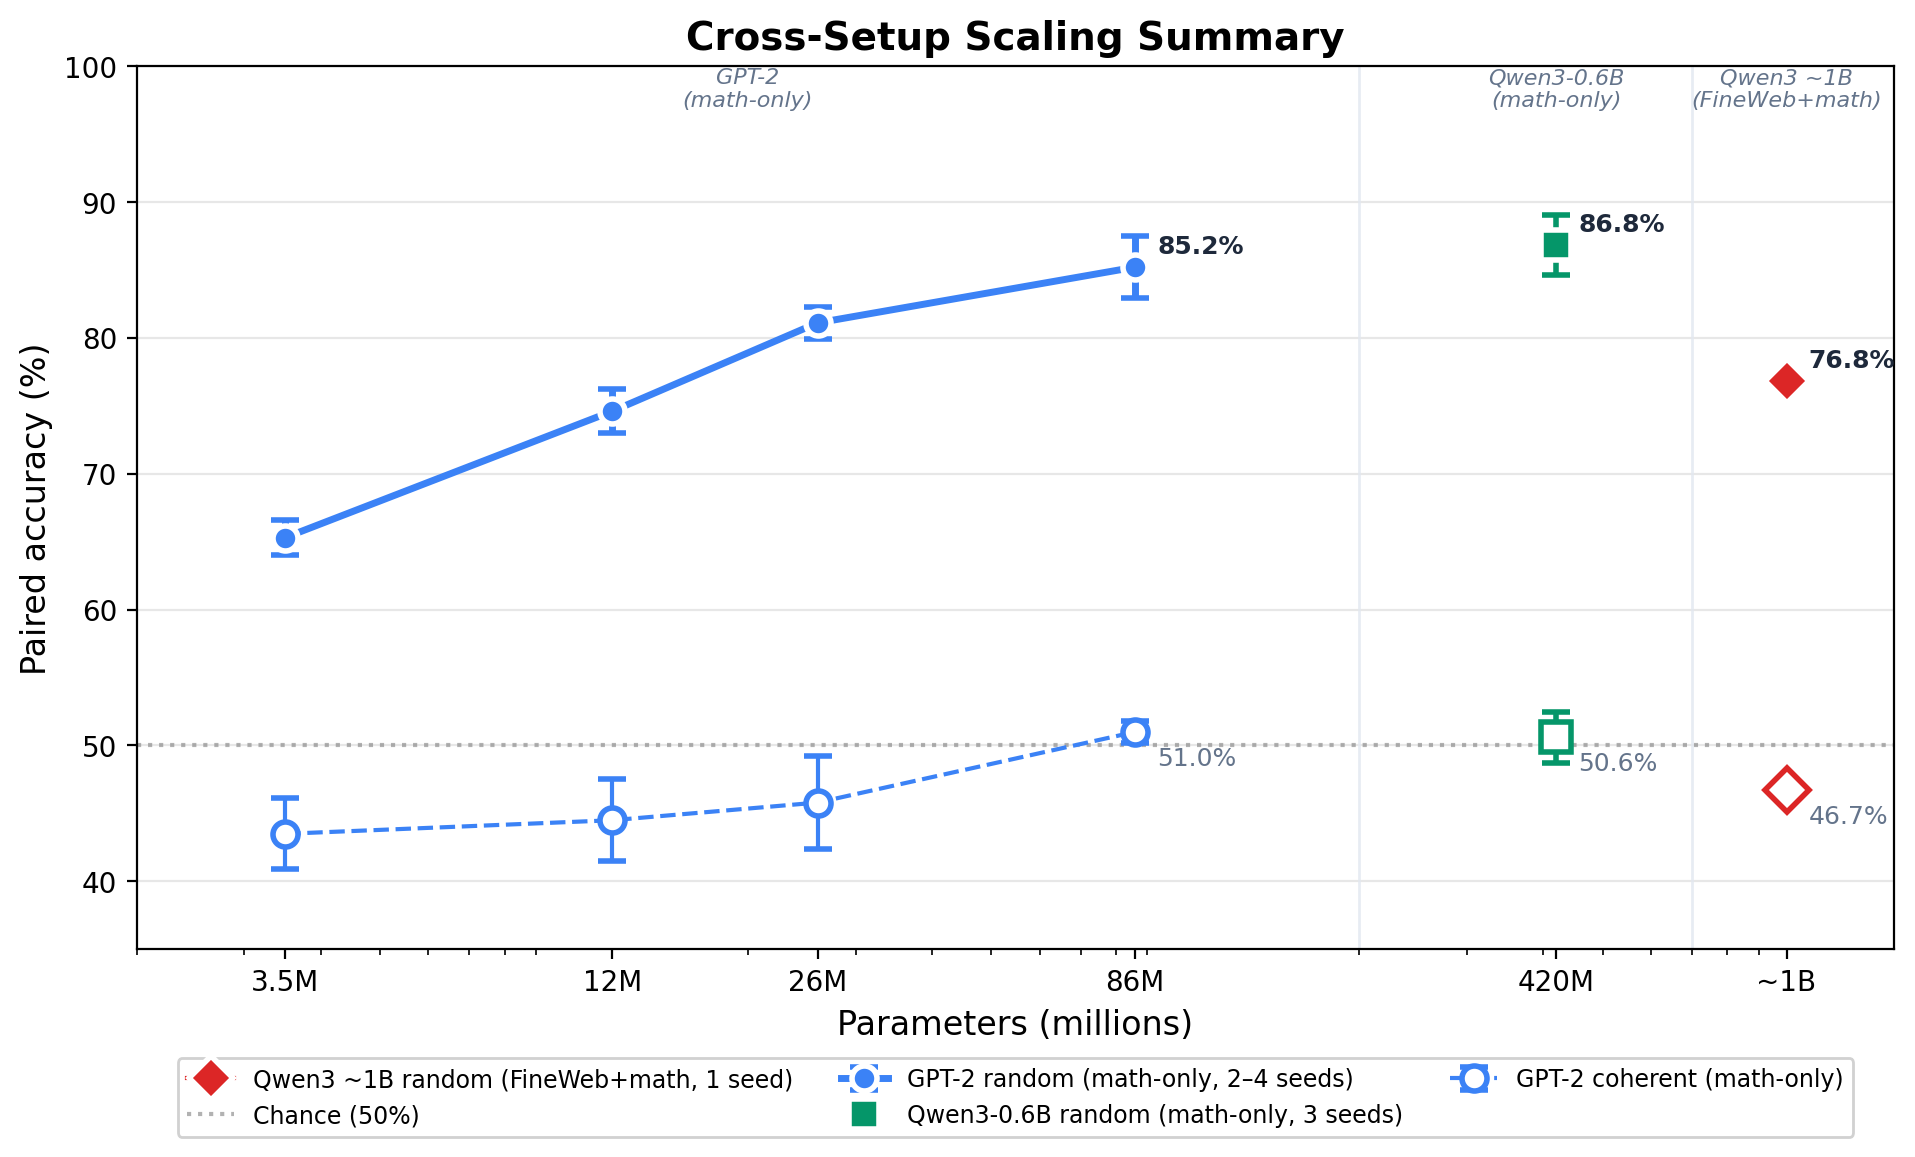
\includegraphics[width=0.62\textwidth]{figure_full_scaling.png}
\caption{Cross-setup pair-accuracy summary: GPT-2 family (3.5M--86M, math-only, 2--4 seeds), Qwen3-0.6B (420M, math-only, 3 seeds), Qwen3-architecture 490M (FineWeb-Edu + 8\% math, 2 seeds). Setups differ in architecture, corpus and seed count, and every point is pair accuracy, which Section~\ref{sec:central} shows overstates the excess above chance about fourfold where both measures exist. Read as directional robustness of the pairwise contrast---not a scaling law, and not the size of the effect.}
\label{fig:qwen}
\end{figure}

%======================================================================
\section{Discussion}
\label{sec:discussion}
%======================================================================

\textbf{Summary of findings.}\quad Two math corpora agree at 86M: a false system whose output the model cannot predict from the problem loses about ten points of probability mass to the correct one ($59.0\%$ denoising, $59.4\%$ standard), and a coherent false rule loses none at any size we tested. Below 86M the two corpora disagree---the standard corpus shows the effect from 12M, the denoising corpus not at all---so the effect is established at one size on two corpora and nowhere below. The generative evaluation, which no splitting argument touches, does separate the conditions at every size. We describe this as a contrast between predictable and unpredictable false systems, and Section~\ref{sec:learnable} identifies that axis directly: holding the false support at a fixed ten strings and varying only whether the model can learn which one applies flips the sign of the preference, from ${+}5$ points for the correct system when the selector is unpredictable to ${-}7$ when it is a learnable digit lookup, with a monotone interpolation between. Predictability---not the description length of the false rule, which the ladder shows does nothing---is what moves it.

\textbf{What we withdraw.}\quad Preference is not graded in the description length of the false system. The two experiments built to show it---competing wrong rules, and a ladder over the number of constants a single wrong rule stores---move pair accuracy by 32 and 16 points while leaving probability mass flat or falling, and their apparent signal is the model's inability to predict which false string will appear, credited to the correct side by a pairwise comparison. Nor do coherent errors fall below chance: that reading was completion length. Nor is the effect present at every scale we tested. These three claims were central to the first version of this work and none of them survives its own control.

\textbf{The role of frequency.}\quad Coherent falsehood needs no frequency advantage to neutralize any preference for the correct answer: at 50/50 the model is at chance, and shifting to 40/60 and 20/80 moves it to 72\% and 90\% preference for the false system. Because the coherent false support is a single string, these numbers are unaffected by splitting. We drop the parallel claim for random errors, which rests on pair accuracy alone.

\textbf{What pair accuracy is good for.}\quad The metric is not worthless---it is a legitimate measure of a ranking behavior, and it is what the surrounding literature reports---but it answers a narrower question than it appears to. When the false side can take more than one form, the correct string competes against a divided opponent, and a model with no preference at all wins. Any experimental design that varies the number of false forms (competing rules, noise ratios, entity substitution, corruption load) varies the metric along with the treatment. We would expect this to affect published results beyond our own wherever contradictory or corrupted data is evaluated pairwise.

\textbf{Implications and scope.}\quad Within these settings, the training objective offers no inherent ``truth compass''. Internally coherent falsehood stays competitive at every size we tested, on both synthetic math and diluted natural text; the preference against incoherent falsehood is real but modest where we can measure it cleanly; and its stronger form (Section~\ref{sec:learnable}) is that a false system the model \emph{can} predict is preferred over the correct one, so what the objective rewards is a learnable, compressible system rather than a true one. That bears on data curation, where coordinated errors would evade diversity-based filtering and a systematic---hence learnable---corruption is exactly the kind this preference favours, and on the reading of hallucination as a corpus-statistics phenomenon \citep{kalai2024calibrated}. All our models remain far below production scale, the identification isolates predictability while leaving the interpretation in terms of compression as an interpretation, and we make no claims about production models.

%======================================================================
\section{Conclusion}
%======================================================================

Measured against everything an error generator can produce, rather than against one sampled error, correctness preference in contradictory training data is smaller than the pairwise metric reports and appears later. At 86M parameters the correct completion holds $59.0\%$ of the probability mass where the pairwise comparison reports $77.6\%$; below 86M the aggregate share shows no preference at all, while pair accuracy already reads 72--89\%. A single coherent false rule is not filtered at any size, architecture or corpus we tested, and this half of the contrast is immune to the objection by construction. Preference is not graded in the description length of the false system: both experiments we built to show that turned out to measure how the false mass is divided. What does move it is predictability---holding the false support at a fixed size and making its selector learnable turns the correct system's small advantage into a preference for the false one, and the effect interpolates with how learnable the selector is. That contrast holds from 420M to a genuine 3.08B parameters. The behavioral finding is a preference for a learnable, internally consistent system over a true one; we report it as such.

%======================================================================
\section*{Limitations}
\label{sec:limitations}
%======================================================================

\textbf{Measurement.}\quad The aggregate share sums probability over the false support the training generator can produce for each problem. It is exact only where that support can be enumerated, which rules out the Wikipedia and natural-text settings, and it is a lower bound rather than a point estimate, since adding strings to the sum can only lower it. It also carries a downward bias that grows as the model gets smaller: on a corpus containing the same problems and no false rule at all, the same 18-mode share reads $99.7\%$ at 86M but $64.1\%$ at 3.5M (Section~\ref{sec:ladder}). Where we report an effect the measure is close to unbiased; where we report none, it is conservative and a small preference could be hidden by the leak. Results elsewhere in the paper that rest on pair accuracy alone are marked in place.

\textbf{Model scale, and the lower end.}\quad Primary experiments use 3.5M--86M parameter models; Section~\ref{sec:qwen1b} extends to 490M on natural text (2 seeds). The scale limitation now runs in both directions. Under the aggregate share the effect is present only at our largest primary size on the denoising corpus ($18.6$, $31.6$, $44.1$, $59.0$ at 3.5M--86M) and from 12M on the standard corpus, so there is exactly one size at which it is established on both, and no evidence that it holds below. At the top end the multi-billion replication we previously named as the next step is now done: on the held-out scale grid, with an enumerable error family and 2 seeds, the random/coherent/learnable contrast holds at a genuine 1.12B, 2.16B and 3.08B parameters (Appendix~\ref{app:scale}). What remains open is the low end---no controlled evidence below 420M except generation---and compute-matched rather than single-pass training at the billion scale.

\textbf{Domain specificity.}\quad Mathematics provides an unusually crisp correct/incorrect distinction and, more importantly here, a false-answer generator whose output support we can enumerate exactly. Wikipedia entity substitution has no such support in general, so its random condition cannot be scored the way the math conditions are. We ran the tractable special case---restricting evaluation to single-entity paragraphs, whose false support is exactly the substituted entity type's pool---and it does not rescue the random condition at trainable scale: that pool runs to ${\sim}2800$ strings, two orders past the math grid's ${\sim}18$, so the family measure's downward leak, calibrated on a clean model trained with no false rule, reaches ${\sim}95$ points below 1B---a clean 86M model reads $5\%$ of the mass on the correct string where it should read ${\sim}100\%$, and the random-trained model sits in the same band ($4\%$), both far under the $0.5$ null. The single-entity coherent support (one false mode, no leak) is length-mismatched instead: only ${\sim}25$ of $384$ problems are token-length-matched, and pooled across all four sizes and both seeds that subset reads $52 \pm 4$ at the $0.5$ null---coherent not filtered on the mass measure either, matching the paired result, but underpowered per cell. So the enumerable-support route quantifies \emph{why} natural text resists this measurement rather than removing the obstacle, and what transfers cleanly remains the coherent result. Domains with competing real-world knowledge systems (conflicting news sources, historical revisionism) remain open.

\textbf{Discriminative vs generative gap.}\quad Pair accuracy (85\%) substantially exceeds generative accuracy (53\%) at large scale, the familiar teacher-forcing gap. Pair accuracy is not a controlled diagnostic of preference: whenever the false side has more than one form, a model reproducing training frequencies wins the comparison. On the denoising corpus at 86M it reports $37.4$~pp of excess above chance where the aggregate share reports $9.0$~pp. We report it only for comparability with prior work.

\textbf{Causal identification.}\quad The two designs the first version offered---the multi-rule experiment (mass $47.9 \to 47.8\%$ at $N{=}1 \to 2$ while pair accuracy jumps 32~pp) and the description-length ladder (flat at 86M: $55.6$, $51.9$, $52.6$, $51.3$)---both confound their treatment with mode count and identify nothing. The learnable-selector control (Section~\ref{sec:learnable}) removes that confound: it fixes the false support at ten strings and varies only whether the selector is learnable, and the preference swings from ${+}5$ points (unpredictable) through the null (partly learnable, \texttt{k2}/\texttt{k3}) to ${-}7$ (a learnable digit lookup), monotone in the realized share. That isolates predictability as the causal axis, which is the identification we said we could not build. Three limits remain and we do not overclaim past them. First, it isolates predictability, not description length: the interpretation that the model prefers the \emph{more compressible} of two systems is consistent with the swing but not measured by it, since a learnable selector is both more predictable and cheaper to store. Second, the realized false support is ten strings, not one, so the design isolates predictability from mode \emph{count} but not from the existence of a small multiplicity; a version holding the realized support at one string while varying its predictability is still open. Third, the below-null readings rest on a matched-competence argument (\texttt{random} and \texttt{learnable} share correct-side training) rather than on a null that is clean below $0.5$; and all of it is one formal-math corpus family.

\textbf{Future directions.}\quad Linear probing for ``truth'' vs ``coherence'' directions in models trained under our conditions could link behavior to internal representations; interactions with RLHF and in-context learning are natural extensions.

\textbf{Ethical considerations.}\quad Internally consistent misinformation can be harder for models to filter than diverse errors; this is a controlled diagnostic finding, not evidence of production-LLM vulnerability. Transparent reporting of such failure modes can inform defensive data curation and evaluation.

%======================================================================
% References
%======================================================================
\bibliographystyle{abbrvnat}
\bibliography{references}

%======================================================================
\appendix
%======================================================================

\section{Reproducibility}
\label{app:reproducibility}

All code, data generation scripts, and evaluation scripts are available at [anonymous repository, included as supplementary material]. Denoising experiments were run on Modal.com T4 GPUs using PyTorch; the control grids of Sections~\ref{sec:central} and \ref{sec:ladder} were rerun on 8${\times}$H100 nodes. Standard math and Wikipedia experiments were run on Apple Mac M4 (36GB) using MLX (v0.31.0). Qwen3-0.6B experiments were run on Modal.com A10G GPUs; the 490M Qwen3-architecture FineWeb-Edu experiments were run on Kaggle T4 GPUs (per the run records; an earlier draft said Modal A100). Over 300 models were trained across all conditions.

\textbf{Released with this paper.}\quad The corpora, the support-enumeration code and the per-run outputs behind both control grids: 64 description-length ladder runs (4 rungs $\times$ 4 sizes $\times$ 4 seeds) plus 8 clean-corpus controls, and 32 denoising runs (2 conditions $\times$ 4 sizes $\times$ 4 seeds). The corpora regenerate byte-identically from their seeds and we publish their SHA-256 checksums; the enumeration script verifies, for every problem, that the error the corpus contains is a member of the enumerated support, and aborts otherwise. Training weights were deleted after evaluation, so only the metric JSON is retained for the cluster grids.

\textbf{Corpus generation examples.}\quad Each problem is generated programmatically and verified by SymPy. Below is a representative training example (denoising, equal random condition):

\begin{verbatim}
Problem: Expand and simplify 3 * (2x + 5) - 4x
Step 1: 3 * (2x + 5) = 6x + 15
Step 2: 6x + 15 - 4x = 2x + 15
Answer: 2x + 15
\end{verbatim}

The corresponding random-error version replaces a derivation step with a plausible but incorrect computation (e.g., \texttt{6x + 15 - 4x = 2x + 11}). In the coherent condition, a systematic rule is applied consistently across all problems of the same type (e.g., for distribution: $a(b+c) = ab + c$ instead of $ab + ac$). The paired test set presents the same prompt with both correct and incorrect completions for NLL comparison.

\section{The MDL Framing, and What It Predicted}
\label{app:mdl}

This appendix records the reasoning that motivated the experimental design, and
what happened to it. All of it describes an idealized two-part MDL learner
\citep{rissanen1978modeling,grunwald2007minimum}, not a theorem about
gradient-descent training.

\textbf{Setup.} A corpus $D$ of $n$ problems, each appearing with an answer from
a correct rule system $T_1$ and one from an alternative $T_2$. The model must
encode \emph{both} clusters---it cannot select one theory and discard the
other---which we model as a latent-source mixture with per-problem assignments
$z_i \in \{1,2\}$:
\[
L(M) + L(D|M) = \underbrace{L(T_1) + L(T_2)}_{\text{theories}} + \underbrace{L(\{z_i\})}_{\text{source assignments}} + \underbrace{\sum_i L(a_i | T_{z_i})}_{\text{answers given sources}}
\]
A learner that internalizes the more compressible theory encodes its answers
cheaply and pays a higher per-token cost for the other cluster.

\textbf{Prediction 1} (random errors): if $T_1$ is compact and $T_2$ is a set of
independent random answers, the correct cluster holds more probability mass.
\emph{Partly borne out.} That quantity is exactly the aggregate share of
Section~\ref{sec:evaluation}. It exceeds $0.5$ at 86M ($59.0\% \pm 0.8$) and
fails at 3.5M--26M ($18.6\%$, $31.6\%$, $44.1\%$), where the model places more
mass on the false support than on the correct string.

\textbf{Prediction 2} (coherent errors): if $L(T_1) \approx L(T_2)$, then at
equal frequency the two clusters receive comparable mass. \emph{Borne out} at
every size, architecture and corpus we tested (Sections~\ref{sec:central},
\ref{sec:wikipedia}, \ref{sec:qwen}).

\textbf{Prediction 3} (multi-rule errors): $N$ compact rules with random
assignment to problems cost an extra $O(n \log N)$ bits for the selector, which
should restore the correct cluster's advantage. \emph{Not borne out.} Mass on
the correct cluster reads $47.9$, $47.8$, $41.8$, $41.9$ and $38.7\%$ at
$N = 1, 2, 3, 5, 10$ (Section~\ref{sec:multirule}), and the ladder of
Section~\ref{sec:ladder}---which varies the number of constants a single false
rule stores while holding the realized false string at one---is flat at 86M
($55.6$, $51.9$, $52.6$, $51.3$). Whatever the selector costs an idealized
learner, it does not move these models' allocation between the clusters.

The graded reading of this framework is therefore refuted by our own
measurement, and only its binary consequence (Prediction 2, and Prediction 1 at
our largest size) survives. One prediction the graded reading did not make, but
the learnability account does, is borne out: the extra cost the mixture pays for
the false cluster is the source-assignment term $L(\{z_i\})$, and that term is
paid only when the assignment $z_i$ cannot be recovered from the problem. Making
it recoverable---the learnable selector of Section~\ref{sec:learnable}---should
remove the cost and let the model commit to the false cluster, and it does: the
correct share drops below the null there while the ladder, which left the
assignment unpredictable at every rung, never moved. So the assignment term, not
the theory-description terms $L(T_1)+L(T_2)$, is what these models are sensitive
to. We report compression as an interpretation of the surviving contrast, not as
a quantity these experiments measure.

\section{Control Grids in Full}
\label{app:controls}

\subsection{Description-Length Ladder, All Sizes}

\begin{table}[h]
\centering
\small
\begin{tabular}{llcccc}
\toprule
Params & Support & $L{=}1$ & $L{=}4$ & $L{=}16$ & $L{=}64$ \\
\midrule
\multirow{2}{*}{3.5M} & realized & $62.6 \pm 2.2$ & $69.2 \pm 2.0$ & $71.8 \pm 2.0$ & $71.9 \pm 1.2$ \\
 & family & $62.6 \pm 2.2$ & $40.5 \pm 2.5$ & $30.8 \pm 1.4$ & $22.3 \pm 1.2$ \\
\midrule
\multirow{2}{*}{12M} & realized & $63.0 \pm 1.4$ & $72.6 \pm 1.4$ & $80.7 \pm 0.9$ & $81.8 \pm 1.2$ \\
 & family & $63.0 \pm 1.4$ & $49.6 \pm 1.9$ & $45.1 \pm 1.8$ & $36.2 \pm 1.8$ \\
\midrule
\multirow{2}{*}{26M} & realized & $57.5 \pm 1.2$ & $68.0 \pm 0.9$ & $77.4 \pm 1.6$ & $81.6 \pm 1.4$ \\
 & family & $57.5 \pm 1.2$ & $50.8 \pm 1.6$ & $51.8 \pm 1.8$ & $43.9 \pm 1.9$ \\
\midrule
\multirow{2}{*}{86M} & realized & $55.6 \pm 0.7$ & $60.7 \pm 1.8$ & $67.2 \pm 0.9$ & $71.8 \pm 1.2$ \\
 & family & $55.6 \pm 0.7$ & $51.9 \pm 1.6$ & $52.6 \pm 0.6$ & $51.3 \pm 1.3$ \\
\bottomrule
\end{tabular}
\caption{Description-length ladder, 4 rungs $\times$ 4 sizes $\times$ 4 seeds (\%). Completion lengths differ by at most $0.043$ tokens across all 64 runs, and the length-matched subset reproduces these values to within $1.1$ points.}
\label{tab:ladder_full}
\end{table}

\begin{table}[h]
\centering
\small
\begin{tabular}{lcccc}
\toprule
Support summed & 3.5M & 12M & 26M & 86M \\
\midrule
Full family, 18 strings & $64.1 \pm 4.4$ & $93.2 \pm 0.6$ & $97.3 \pm 1.3$ & $99.7 \pm 0.0$ \\
Realized, 1 string & $95.1 \pm 1.0$ & $99.6 \pm 0.1$ & $99.9 \pm 0.0$ & $100.0 \pm 0.0$ \\
\bottomrule
\end{tabular}
\caption{Calibration control: the same measures applied to models trained on a corpus containing the same problems and \emph{no false rule anywhere} (2 seeds, \%). The true value is 100 by construction, so the shortfall is the measure's downward bias. It is $0.3$ points at 86M and $36$ points at 3.5M. The $\pm 4.4$ at 3.5M is a spread of $59.7$ to $68.5$ across two seeds.}
\label{tab:clean_control}
\end{table}

\subsection{Multi-Rule Sweep}

\begin{figure}[h]
\centering
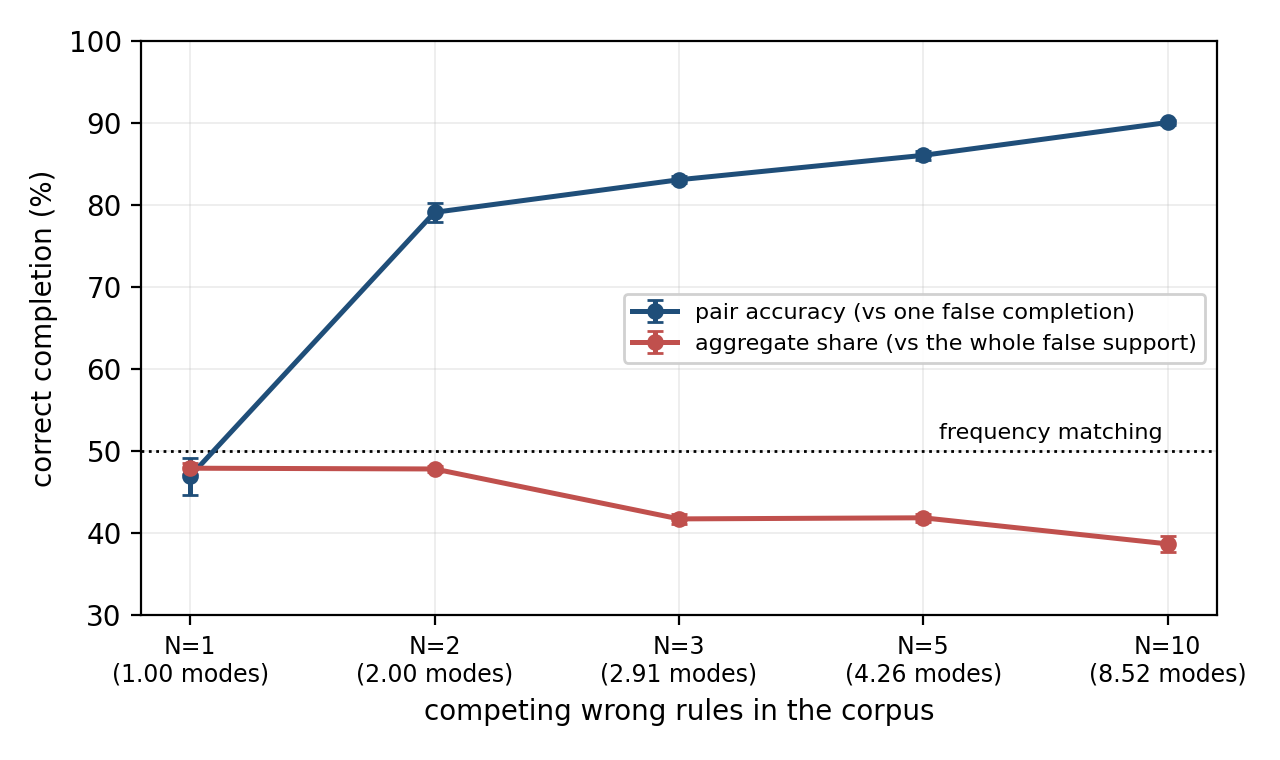
\includegraphics[width=0.7\textwidth]{figure_multirule_control.png}
\caption{Multi-rule errors under both measures (tiny, 4 seeds). Pair accuracy rises monotonically with the number of distinct false modes while the model's allocation between the correct and false clusters does not move at $N{=}1 \to 2$ and declines thereafter. X-axis is categorical.}
\label{fig:multirule}
\end{figure}

\subsection{Standard Corpus, Aggregate Share}

\begin{table}[h]
\centering
\small
\begin{tabular}{lcccc}
\toprule
Condition & 3.5M & 12M & 26M & 86M \\
\midrule
Random (5.51 modes) & $50.2 \pm 0.7$ & $57.6 \pm 0.2$ & $59.0 \pm 0.3$ & $\mathbf{59.4 \pm 0.6}$ \\
\quad equal length & $53.2 \pm 1.1$ & $57.9 \pm 0.4$ & $57.8 \pm 0.2$ & $58.5 \pm 0.7$ \\
Coherent (1 mode) & $47.3 \pm 0.7$ & $49.2 \pm 0.4$ & $50.0 \pm 0.4$ & $50.1 \pm 0.1$ \\
\quad equal length & $49.3 \pm 0.7$ & $49.5 \pm 0.4$ & $49.9 \pm 0.4$ & $49.7 \pm 0.2$ \\
\bottomrule
\end{tabular}
\caption{Aggregate share on the standard (non-denoising) corpus, 4 seeds (\%); $n{=}1101$ problems for random and $915$ for coherent, of which $359$ and $561$ are length-matched. The $59.4$ at 86M is the independent replication of the $59.0$ obtained on the denoising corpus. Per-seed bootstrap intervals for the random condition lie entirely above $0.5$ at 12M, 26M and 86M. The coherent intervals contain $0.5$ from 26M upward; at 3.5M all four lie entirely below it, and at 12M one of four does, consistent with the length account of Section~\ref{sec:central}.}
\label{tab:standard_share}
\end{table}

\section{The Held-Out Scale Grid and the Learnable-Selector Control}
\label{app:scale}

This grid trains one model per condition on 500k problems for 5000 steps at batch
32 ($0.44$ epochs, so no problem is seen twice) and evaluates on ${\approx}2.5$k
held-out problems disjoint from training by a hash of the problem parameters. It
is the measurement behind Sections~\ref{sec:qwen} and \ref{sec:learnable} and the
billion-scale replication. Because each problem is written once---correct with
probability $0.5$, otherwise one false string---the frequency-matching null for
the family share is exactly $0.500$ (a marginal correction from arithmetic
problems that render identically in every mode raises it to at most $0.513$; we
read the band $[50.0, 51.3]$). We report the length-matched subset, on which the
completion-length confound of Section~\ref{sec:central} is removed.

\textbf{A null of indifference is also a null of competence.} Every null here
describes a model that both lacks a preference \emph{and} can compute the correct
answer; a model that prefers truth but has not learned the arithmetic reads below
it too. So a below-null cell is not on its own evidence of a preference for the
false side. Only excursions above the band are unambiguous---except where a
matched-competence contrast is available, as in the learnable control below,
where \texttt{random} and \texttt{learnable} share their correct-side training and
so cannot differ in competence.

\begin{table}[h]
\centering\small
\begin{tabular}{lccccccc}
\toprule
 & 3.5M & 12M & 26M & 86M & 202M & 418M & 474M \\
\midrule
random (eqlen)   & $15.1$ & $32.8$ & $40.4$ & $45.5$ & $48.5$ & $\mathbf{56.8}$ & $\mathbf{54.9}$ \\
coherent (eqlen) & $49.4$ & $51.6$ & $51.2$ & $52.4$ & $51.9$ & $50.2$ & $49.9$ \\
clean (full)     & ---    & ---    & ---    & $80.9$ & $91.7$ & $99.4$ & $99.2$ \\
clean (eqlen)    & ---    & ---    & ---    & $91.0$ & $92.2$ & $97.9$ & $97.2$ \\
\bottomrule
\end{tabular}
\caption{Held-out scale grid, family measure, \% mass on the correct completion (null $50$). GPT-2 sizes 3.5M--202M (4 seeds), Qwen3 sizes 418M/474M (4 seeds on random and coherent). The above-null random cells appear only at 418M--474M; coherent sits at the null throughout. \emph{clean} trains on the same problems with no false rule anywhere: its shortfall below the ideal $100$ is the measure's downward leak, which is monotone in scale and never lifts a value \emph{above} the ideal, so it cannot manufacture the above-null random cells. The leak is also architecture-dependent---a same-size 413M GPT-2 leaks like a 202M GPT-2 (clean eqlen $93.5$) and its random cell straddles the null ($52.3/50.1$), where Qwen3 is tight and clearly above.}
\label{tab:scale_grid}
\end{table}

\textbf{The learnable-selector control (Section~\ref{sec:learnable}), full grid.}
The false answer is $a{\cdot}b + T[\,s(p)\bmod 10\,]$ with $T$ a fixed 10-entry
table, so the false support is ten strings per problem in every row; only the
selector $s(p)$ changes. Family share is the length-matched subset; \emph{realized}
scores the correct completion against the single false string the corpus used.

\begin{table}[h]
\centering\small
\begin{tabular}{lcccc}
\toprule
 & \multicolumn{2}{c}{418M} & \multicolumn{2}{c}{474M} \\
\cmidrule(lr){2-3}\cmidrule(lr){4-5}
Selector $s(p)$ & family & realized & family & realized \\
\midrule
\texttt{learnable} (1 digit)   & $44.7 \pm 1.0$ & ${\approx}65$ & $43.4 \pm 0.7$ & $66$ \\
\texttt{k2} (2 digits)         & $48.6 \pm 0.0$ & $85.9 \pm 0.6$ & $49.2 \pm 0.1$ & $88.6 \pm 0.1$ \\
\texttt{k3} (3 digits)         & $47.6 \pm 1.4$ & $89.7 \pm 1.1$ & $48.8 \pm 0.1$ & $91.6 \pm 0.2$ \\
\texttt{learnable\_mod} (all)  & ---            & ---           & $55.4$         & $93$ \\
\bottomrule
\end{tabular}
\caption{Learnable-selector gradient (Qwen3, family measure on the length-matched subset, null $50$). \texttt{learnable} is 4 seeds, \texttt{k2}/\texttt{k3} are 2 seeds, \texttt{learnable\_mod} 2 seeds at 474M. As the selector is made to depend on more digits it is fitted less (realized share climbs $65 \to 89 \to 92$), and the family share climbs off the below-null value to the null. \texttt{learnable\_mod} (sum of all operands mod $n$) is deterministic but never learned, so it reads like \texttt{random}; it changes the realized mode count, so it anchors the unlearnable end as a direction rather than a matched-diversity point.}
\label{tab:learnable_full}
\end{table}

\textbf{Billion-scale replication.} Genuine Qwen3-architecture models at 1.12B,
2.16B and 3.08B parameters (bf16, gradient checkpointing; 2 seeds each) reproduce
the full contrast on the controlled measure (Table~\ref{tab:billions}). A 4.39B
configuration exceeds one H100's memory with fp32 optimizer states and is not run.

\begin{table}[h]
\centering\small
\begin{tabular}{lccccc}
\toprule
Params & random & coherent & learnable & \texttt{learnable\_mod} & clean \\
\midrule
1.12B & $55.5$ & $49.5$ & $43.8$ & --- & $98.1$ \\
2.16B & $54.5$ & $50.7$ & $43.1$ & $54.2$ & $96.4$ \\
3.08B & $56.6$ & $49.3$ & $43.7$ & $54.6$ & $99.0$ \\
\bottomrule
\end{tabular}
\caption{Billion-scale replication (family measure, length-matched subset, null $50$, 2 seeds). Correct system above the null against an unpredictable false family, coherent at the null, learnable false selector below the null (preferred), \texttt{learnable\_mod} unlearned and so at the random level, clean calibration above $96\%$ at every size. \texttt{learnable\_mod} was not run at 1.12B.}
\label{tab:billions}
\end{table}

\section{Compression Measure (gzip)}
\label{app:compression}

To operationalize the MDL argument, we measure compression ratios (gzip level 9) on concatenated correct vs incorrect completions from each paired test set.

\begin{table}[h]
\centering
\small
\begin{tabular}{lcccc}
\toprule
Condition & Correct & Incorrect & Delta & Paired Accuracy \\
\midrule
random 50/50     & 0.1627 & 0.1639 & $+0.0012$ & 79.5\% \\
coherent 50/50   & 0.1656 & 0.1658 & $+0.0002$ & 47.2\% \\
contradictory    & 0.1745 & 0.1744 & $-0.0001$ & 49.0\% \\
multirule $N{=}2$  & 0.1671 & 0.1710 & $+0.0038$ & 77.6\% \\
multirule $N{=}3$  & 0.1669 & 0.1722 & $+0.0053$ & 82.8\% \\
multirule $N{=}5$  & 0.1672 & 0.1730 & $+0.0057$ & 84.8\% \\
multirule $N{=}10$ & 0.1676 & 0.1752 & $+0.0076$ & 88.3\% \\
world random     & 0.0370 & 0.0516 & $+0.0146$ & 57.7\% \\
world coherent   & 0.0374 & 0.0384 & $+0.0010$ & 46.6\% \\
\bottomrule
\end{tabular}
\caption{Compression ratio (gzip) and paired accuracy across all 9 conditions. Spearman $\rho = 0.67$; two-sided $p = 0.05$ under the $t$ approximation and $0.06$ by exact permutation, i.e.\ not significant at the conventional level.}
\label{tab:compression}
\end{table}

The multi-rule accuracies here ($77.6$, $82.8$, $84.8$, $88.3$) come from the paired evaluation on the held-out paired test set; Table~\ref{tab:multirule} reports the same conditions scored on the enumerated support ($79.1$, $83.1$, $86.1$, $90.1$). Both are pair accuracies on the same checkpoints, differing only in which problems and which false completions they are computed over.

Conditions with larger compression gaps show higher pair accuracy. This correlation should now be read with care: four of the nine points are the multi-rule conditions, whose pair accuracy is known to be inflated by mass splitting (Section~\ref{sec:multirule}), and their compression deltas ($+0.0038$ to $+0.0076$) grow monotonically with the number of rules, because adding rules adds text diversity. The same variable therefore moves both axes, and the correlation cannot be read as evidence that compressibility drives preference. Recomputed against aggregate share for the multi-rule points ($47.9$, $47.8$, $41.8$, $41.9$, $38.7$), the relationship disappears. We retain the appendix as a record of the measurement, not as support for the hypothesis.

\section{Standard (Non-Denoising) Experiments}
\label{app:standard}

\subsection{Standard Corpus Design}

In the standard setup, each problem appears once with either a correct or incorrect solution. The two groups do not share prompts.

\subsection{Standard vs Denoising}

\begin{table}[h]
\centering
\small
\begin{tabular}{lccc}
\toprule
Size & Standard & Denoising & Gap \\
\midrule
tiny   & 79.5\% & 65.3\% & $-14.2$ pp \\
small  & 86.2\% & 74.6\% & $-11.6$ pp \\
medium & 87.1\% & 81.1\% & $-6.0$ pp \\
large  & 88.3\% & 85.2\% & $-3.1$ pp \\
\bottomrule
\end{tabular}
\caption{Standard vs denoising accuracy (50/50 random). The gap closes with scale.}
\label{tab:standard_vs_denoising}
\end{table}

The denoising setup is harder (within-problem contradiction vs across-corpus mixing), but the gap closes with scale.

\subsection{Frequency Effects}

\begin{table}[h]
\centering
\small
\begin{tabular}{cccc}
\toprule
Proportion & Random & Coherent & False pref. \\
\midrule
50/50 & 79.5\% & 47.2\% & 52.8\% \\
40/60 & 79\% & 27.8\% & 72.2\% \\
30/70 & 75\% & 14.7\% & 85.3\% \\
20/80 & 69\% & 9.6\%  & 90.4\% \\
10/90 & 67\% & --     & -- \\
\bottomrule
\end{tabular}
\caption{Random vs coherent accuracy across proportions (standard, tiny). Random: truth bias persists at 10/90. Coherent: the model follows pure frequency. ``False pref.'' = $1 - \text{coherent accuracy}$, i.e., the fraction of pairs where the model prefers the coherent false completion.}
\label{tab:frequency}
\end{table}

\subsection{Noise Tolerance}

\begin{table}[h]
\centering
\small
\begin{tabular}{lccccc}
\toprule
Condition & Ratio & Tiny & Small & Medium & Large \\
\midrule
Equal random & 1:1 & 65.3\% & 74.6\% & 81.1\% & 85.2\% \\
2:1 noise    & 1:2 & 59.0\% & 68.6\% & 73.6\% & 75.2\% \\
4:1 noise    & 1:4 & 56.6\% & 64.9\% & 66.6\% & 65.8\% \\
\bottomrule
\end{tabular}
\caption{Paired accuracy at increasing noise ratios (denoising). Accuracy degrades gracefully; at 4:1 noise, it plateaus at medium/large.}
\label{tab:noise}
\end{table}

\subsection{NLL Distribution}

Random errors produce a right-skewed per-pair NLL difference (mean $+0.048$, median $+0.025$, 81.5\% positive). Coherent errors produce a symmetric distribution (45.5\% positive). This explains why pair accuracy and mean $\Delta\text{Loss}$ can diverge. The coherent distribution's centre sits slightly below $0.5$ because the coherent false completions are on average $0.58$ tokens shorter than the correct ones; on length-matched pairs the values move to $46.7$--$49.3\%$ (Section~\ref{sec:central}).

\section{Additional Transfer Experiments}
\label{app:transfer}

\subsection{Synthetic World}

A synthetic world with 50 entities, 4 types, 15 deterministic rules. Random 50/50: $57.7\% \pm 1.7\%$. Coherent 50/50: $46.6\% \pm 1.7\%$. Per-type: minerals best (68.7\%), potions near chance (49.1\%).

\subsection{Wikipedia Per-Entity-Type}

Entity-level breakdowns suggest that the pairwise effect is strongest when substitutions disrupt geographically constrained co-occurrence patterns, and weakest for numeric entities. The per-type samples are small---LOC has 45 pairs, so its $82.2\%$ carries a 95\% binomial interval of roughly $\pm 11$~pp---and these are pair-accuracy values on a multi-mode false support, so the ordering is suggestive rather than established.

\begin{table}[h]
\centering
\small
\begin{tabular}{lcc}
\toprule
Entity Type & $N$ Pairs & Accuracy \\
\midrule
LOC      & 45  & 82.2\% \\
NORP     & 197 & 78.7\% \\
GPE      & 301 & 77.1\% \\
PERSON   & 402 & 69.9\% \\
ORG      & 664 & 65.2\% \\
CARDINAL & 172 & 61.0\% \\
\bottomrule
\end{tabular}
\caption{Wikipedia accuracy by entity type (random substitution, averaged across sizes).}
\label{tab:wiki_entity}
\end{table}

\subsection{Cross-Domain Falsification}

Adding correct cross-domain tasks to a coherent corpus selectively increases derivative accuracy ($35\% \to 56\%$ at 25\%). The effect is non-monotonic (drops at 50\% due to dilution).

\section{Robustness Checks}
\label{app:robustness}

\subsection{BPE Tokenization}

\begin{table}[h]
\centering
\small
\begin{tabular}{llcc}
\toprule
Setup & Tokenizer & Random (pair acc.) & Coherent (pair acc.) \\
\midrule
Standard  & Char & 79.5\% & 47.2\% \\
Standard  & BPE  & $\mathbf{85.6\%}$ & 45.9\% \\
Denoising & Char & 65.3\% & 43.5\% \\
Denoising & BPE  & $\mathbf{75.9\%}$ & 49.3\% \\
\bottomrule
\end{tabular}
\caption{BPE vs char-level (tiny, 4 seeds). The effect survives BPE and strengthens for random errors.}
\label{tab:bpe}
\end{table}

\subsection{Chained Verification}
\label{app:chained}

Embedding cross-domain verification dependencies in coherent-error tasks restores truth bias but exhibits inverse scaling across 10 models (4 tiny, 4 small, 2 large):

\begin{table}[h]
\centering
\small
\begin{tabular}{lccc}
\toprule
Size & Paired Accuracy & Seeds & Standard coherent baseline \\
\midrule
tiny (3.5M)  & $70.9\% \pm 1.2\%$ & 4 & $47.2\%$ \\
small (12M)  & $64.2\% \pm 1.5\%$ & 4 & $49.6\%$ \\
large (86M)  & $60.6\% \pm 1.2\%$ & 2 & $51.4\%$ \\
\bottomrule
\end{tabular}
\caption{Chained-verification pair accuracy against the standard-setup coherent baseline measured on the same corpus family (4 seeds; the earlier version of this table printed the \emph{denoising} coherent values here by mistake). Pair accuracy only; the aggregate share was not measured for this condition.}
\label{tab:chained}
\end{table}

The decline with scale should not be read as an inverse-scaling result. The gap between pair accuracy and the aggregate share shrinks with model size wherever we computed both ($53.1$, $52.5$, $45.1$ and $28.4$~pp at 3.5M, 12M, 26M and 86M on the denoising corpus), which alone would produce a declining pair-accuracy trend on a condition where only pair accuracy is available. We report the numbers and do not interpret the trend.

\subsection{Learning Curves}

All sizes reach behavioral plateau by step 3000--4000. The large model reaches 90.4\% at step 3000 and holds 86.4\% and 87.8\% at steps 4000 and 5000. This check rules out an early-stopping artifact; the underlying logs and plotting script are included in the supplementary material.

\section{Per-Seed Details}
\label{app:seeds}

Tables~\ref{tab:seeds_random}--\ref{tab:seeds_coherent} report per-seed pair accuracy for the core denoising conditions as originally run, where the 86M row has two seeds. The control grid of Section~\ref{sec:central} reruns all four sizes with four seeds each on regenerated corpora that match the originals byte for byte (SHA-256 published with the release), and its 86M row therefore supersedes these two-seed entries. Per-run outputs for every cell of both control grids are released; per-seed breakdowns for multi-rule, Wikipedia, and Qwen3 experiments are in the supplementary code repository (evaluation logs per model).

\begin{table}[h]
\centering
\small
\begin{tabular}{lccccc}
\toprule
Size & Seed 1 & Seed 2 & Seed 3 & Seed 4 & Mean \\
\midrule
tiny   & 64.2\% & 64.1\% & 67.0\% & 65.8\% & 65.3\% \\
small  & 75.1\% & 76.3\% & 72.6\% & 74.2\% & 74.6\% \\
medium & 79.6\% & 80.9\% & 82.4\% & 81.3\% & 81.1\% \\
large  & 83.5\% & 86.8\% & --     & --     & 85.2\% \\
\bottomrule
\end{tabular}
\caption{Denoising equal random, per-seed accuracy.}
\label{tab:seeds_random}
\end{table}

\begin{table}[h]
\centering
\small
\begin{tabular}{lccccc}
\toprule
Size & Seed 1 & Seed 2 & Seed 3 & Seed 4 & Mean \\
\midrule
tiny   & 40.2\% & 44.3\% & 46.3\% & 43.0\% & 43.5\% \\
small  & 44.8\% & 45.3\% & 40.3\% & 47.4\% & 44.5\% \\
medium & 45.8\% & 40.9\% & 47.7\% & 48.6\% & 45.8\% \\
large  & 51.6\% & 50.4\% & --     & --     & 51.0\% \\
\bottomrule
\end{tabular}
\caption{Denoising equal coherent, per-seed accuracy.}
\label{tab:seeds_coherent}
\end{table}

\clearpage

%======================================================================
% NeurIPS Paper Checklist (official format)
%======================================================================
\section*{NeurIPS Paper Checklist}

\begin{enumerate}

\item {\bf Claims}
    \item[] Question: Do the main claims made in the abstract and introduction accurately reflect the paper's contributions and scope?
    \item[] Answer: \answerYes{}
    \item[] Justification: The primary metric is aggregate share against the enumerated false support, whose null is exactly 0.500 on our corpora. The abstract and introduction state that the effect is established at 86M on two corpora and not below, that pair-accuracy results elsewhere in the paper are uncontrolled and overstate the excess above chance by a factor of three to four, and that the multi-rule and description-length experiments are reported as negative controls rather than as evidence for a mechanism. Claims that appeared in the first version of this work and did not survive their own controls are named and withdrawn in Sections~\ref{sec:multirule}, \ref{sec:ladder} and \ref{sec:discussion}.
    \item[] Guidelines:
    \begin{itemize}
        \item The answer \answerNA{} means that the abstract and introduction do not include the claims made in the paper.
        \item The abstract and/or introduction should clearly state the claims made, including the contributions made in the paper and important assumptions and limitations. A \answerNo{} or \answerNA{} answer to this question will not be perceived well by the reviewers.
        \item The claims made should match theoretical and experimental results, and reflect how much the results can be expected to generalize to other settings.
        \item It is fine to include aspirational goals as motivation as long as it is clear that these goals are not attained by the paper.
    \end{itemize}

\item {\bf Limitations}
    \item[] Question: Does the paper discuss the limitations of the work performed by the authors?
    \item[] Answer: \answerYes{}
    \item[] Justification: A dedicated Limitations section discusses model scale, domain specificity, discriminative vs generative gap, seed counts, and causal identification.
    \item[] Guidelines:
    \begin{itemize}
        \item The answer \answerNA{} means that the paper has no limitation while the answer \answerNo{} means that the paper has limitations, but those are not discussed in the paper.
        \item The authors are encouraged to create a separate ``Limitations'' section in their paper.
        \item The paper should point out any strong assumptions and how robust the results are to violations of these assumptions (e.g., independence assumptions, noiseless settings, model well-specification, asymptotic approximations only holding locally). The authors should reflect on how these assumptions might be violated in practice and what the implications would be.
        \item The authors should reflect on the scope of the claims made, e.g., if the approach was only tested on a few datasets or with a few runs. In general, empirical results often depend on implicit assumptions, which should be articulated.
        \item The authors should reflect on the factors that influence the performance of the approach. For example, a facial recognition algorithm may perform poorly when image resolution is low or images are taken in low lighting. Or a speech-to-text system might not be used reliably to provide closed captions for online lectures because it fails to handle technical jargon.
        \item The authors should discuss the computational efficiency of the proposed algorithms and how they scale with dataset size.
        \item If applicable, the authors should discuss possible limitations of their approach to address problems of privacy and fairness.
        \item While the authors might fear that complete honesty about limitations might be used by reviewers as grounds for rejection, a worse outcome might be that reviewers discover limitations that aren't acknowledged in the paper. The authors should use their best judgment and recognize that individual actions in favor of transparency play an important role in developing norms that preserve the integrity of the community. Reviewers will be specifically instructed to not penalize honesty concerning limitations.
    \end{itemize}

\item {\bf Theory assumptions and proofs}
    \item[] Question: For each theoretical result, does the paper provide the full set of assumptions and a complete (and correct) proof?
    \item[] Answer: \answerNA{}
    \item[] Justification: The paper does not claim formal theoretical results. Appendix~\ref{app:mdl} presents three MDL-motivated predictions with proof sketches for an idealized learner, explicitly marked as informal predictions rather than formal theorems about neural network training. The paper is primarily empirical.
    \item[] Guidelines:
    \begin{itemize}
        \item The answer \answerNA{} means that the paper does not include theoretical results.
        \item All the theorems, formulas, and proofs in the paper should be numbered and cross-referenced.
        \item All assumptions should be clearly stated or referenced in the statement of any theorems.
        \item The proofs can either appear in the main paper or the supplemental material, but if they appear in the supplemental material, the authors are encouraged to provide a short proof sketch to provide intuition.
        \item Inversely, any informal proof provided in the core of the paper should be complemented by formal proofs provided in appendix or supplemental material.
        \item Theorems and Lemmas that the proof relies upon should be properly referenced.
    \end{itemize}

    \item {\bf Experimental result reproducibility}
    \item[] Question: Does the paper fully disclose all the information needed to reproduce the main experimental results of the paper to the extent that it affects the main claims and/or conclusions of the paper (regardless of whether the code and data are provided or not)?
    \item[] Answer: \answerYes{}
    \item[] Justification: All hyperparameters, model architectures, data generation procedures, evaluation protocols, and random seeds are specified in Section~\ref{sec:methodology} and Appendix~\ref{app:reproducibility}. Full generation templates are included in supplementary material.
    \item[] Guidelines:
    \begin{itemize}
        \item The answer \answerNA{} means that the paper does not include experiments.
        \item If the paper includes experiments, a \answerNo{} answer to this question will not be perceived well by the reviewers: Making the paper reproducible is important, regardless of whether the code and data are provided or not.
        \item If the contribution is a dataset and\slash or model, the authors should describe the steps taken to make their results reproducible or verifiable.
        \item Depending on the contribution, reproducibility can be accomplished in various ways. For example, if the contribution is a novel architecture, describing the architecture fully might suffice, or if the contribution is a specific model and empirical evaluation, it may be necessary to either make it possible for others to replicate the model with the same dataset, or provide access to the model. In general. releasing code and data is often one good way to accomplish this, but reproducibility can also be provided via detailed instructions for how to replicate the results, access to a hosted model (e.g., in the case of a large language model), releasing of a model checkpoint, or other means that are appropriate to the research performed.
        \item While NeurIPS does not require releasing code, the conference does require all submissions to provide some reasonable avenue for reproducibility, which may depend on the nature of the contribution. For example
        \begin{enumerate}
            \item If the contribution is primarily a new algorithm, the paper should make it clear how to reproduce that algorithm.
            \item If the contribution is primarily a new model architecture, the paper should describe the architecture clearly and fully.
            \item If the contribution is a new model (e.g., a large language model), then there should either be a way to access this model for reproducing the results or a way to reproduce the model (e.g., with an open-source dataset or instructions for how to construct the dataset).
            \item We recognize that reproducibility may be tricky in some cases, in which case authors are welcome to describe the particular way they provide for reproducibility. In the case of closed-source models, it may be that access to the model is limited in some way (e.g., to registered users), but it should be possible for other researchers to have some path to reproducing or verifying the results.
        \end{enumerate}
    \end{itemize}


\item {\bf Open access to data and code}
    \item[] Question: Does the paper provide open access to the data and code, with sufficient instructions to faithfully reproduce the main experimental results, as described in supplemental material?
    \item[] Answer: \answerYes{}
    \item[] Justification: Anonymous repository included as supplementary material with full code for data generation, training, and evaluation.
    \item[] Guidelines:
    \begin{itemize}
        \item The answer \answerNA{} means that paper does not include experiments requiring code.
        \item Please see the NeurIPS code and data submission guidelines (\url{https://neurips.cc/public/guides/CodeSubmissionPolicy}) for more details.
        \item While we encourage the release of code and data, we understand that this might not be possible, so \answerNo{} is an acceptable answer. Papers cannot be rejected simply for not including code, unless this is central to the contribution (e.g., for a new open-source benchmark).
        \item The instructions should contain the exact command and environment needed to run to reproduce the results. See the NeurIPS code and data submission guidelines (\url{https://neurips.cc/public/guides/CodeSubmissionPolicy}) for more details.
        \item The authors should provide instructions on data access and preparation, including how to access the raw data, preprocessed data, intermediate data, and generated data, etc.
        \item The authors should provide scripts to reproduce all experimental results for the new proposed method and baselines. If only a subset of experiments are reproducible, they should state which ones are omitted from the script and why.
        \item At submission time, to preserve anonymity, the authors should release anonymized versions (if applicable).
        \item Providing as much information as possible in supplemental material (appended to the paper) is recommended, but including URLs to data and code is permitted.
    \end{itemize}


\item {\bf Experimental setting/details}
    \item[] Question: Does the paper specify all the training and test details (e.g., data splits, hyperparameters, how they were chosen, type of optimizer) necessary to understand the results?
    \item[] Answer: \answerYes{}
    \item[] Justification: See Section~\ref{sec:models} (optimizer, lr, schedule, batch size, steps) and Appendix~\ref{app:reproducibility} (corpus examples, hardware). Train/test separation is guaranteed by seed: test problems use a different seed (999) than training.
    \item[] Guidelines:
    \begin{itemize}
        \item The answer \answerNA{} means that the paper does not include experiments.
        \item The experimental setting should be presented in the core of the paper to a level of detail that is necessary to appreciate the results and make sense of them.
        \item The full details can be provided either with the code, in appendix, or as supplemental material.
    \end{itemize}

\item {\bf Experiment statistical significance}
    \item[] Question: Does the paper report error bars suitably and correctly defined or other appropriate information about the statistical significance of the experiments?
    \item[] Answer: \answerYes{}
    \item[] Justification: All $\pm$ values are standard deviations across random seeds (not standard errors). $p$-values are computed via Wilcoxon signed-rank test (one-sided) on per-pair NLL differences; bootstrap 95\% CIs (10{,}000 resamples) are used for confidence intervals. The number of seeds is reported for every condition. Per-seed breakdowns for the core denoising conditions are provided in Appendix~\ref{app:seeds}. For the 490M FineWeb-Edu experiment (2 seeds), the reported values are pair accuracy on an enumeration-free support and are marked as descriptive.
    \item[] Guidelines:
    \begin{itemize}
        \item The answer \answerNA{} means that the paper does not include experiments.
        \item The authors should answer \answerYes{} if the results are accompanied by error bars, confidence intervals, or statistical significance tests, at least for the experiments that support the main claims of the paper.
        \item The factors of variability that the error bars are capturing should be clearly stated (for example, train/test split, initialization, random drawing of some parameter, or overall run with given experimental conditions).
        \item The method for calculating the error bars should be explained (closed form formula, call to a library function, bootstrap, etc.)
        \item The assumptions made should be given (e.g., Normally distributed errors).
        \item It should be clear whether the error bar is the standard deviation or the standard error of the mean.
        \item It is OK to report 1-sigma error bars, but one should state it. The authors should preferably report a 2-sigma error bar than state that they have a 96\% CI, if the hypothesis of Normality of errors is not verified.
        \item For asymmetric distributions, the authors should be careful not to show in tables or figures symmetric error bars that would yield results that are out of range (e.g., negative error rates).
        \item If error bars are reported in tables or plots, the authors should explain in the text how they were calculated and reference the corresponding figures or tables in the text.
    \end{itemize}

\item {\bf Experiments compute resources}
    \item[] Question: For each experiment, does the paper provide sufficient information on the computer resources (type of compute workers, memory, time of execution) needed to reproduce the experiments?
    \item[] Answer: \answerYes{}
    \item[] Justification: See Appendix~\ref{app:reproducibility}: approximately 150 GPU-hours total on Modal.com T4/A10G/A100 GPUs and Apple M4 Pro (36GB). Hardware is specified per experiment type.
    \item[] Guidelines:
    \begin{itemize}
        \item The answer \answerNA{} means that the paper does not include experiments.
        \item The paper should indicate the type of compute workers CPU or GPU, internal cluster, or cloud provider, including relevant memory and storage.
        \item The paper should provide the amount of compute required for each of the individual experimental runs as well as estimate the total compute.
        \item The paper should disclose whether the full research project required more compute than the experiments reported in the paper (e.g., preliminary or failed experiments that didn't make it into the paper).
    \end{itemize}

\item {\bf Code of ethics}
    \item[] Question: Does the research conducted in the paper conform, in every respect, with the NeurIPS Code of Ethics \url{https://neurips.cc/public/EthicsGuidelines}?
    \item[] Answer: \answerYes{}
    \item[] Justification: The research uses only synthetic data and publicly available Wikipedia text. No human subjects, no private data, no dual-use concerns beyond those discussed in Ethical Considerations.
    \item[] Guidelines:
    \begin{itemize}
        \item The answer \answerNA{} means that the authors have not reviewed the NeurIPS Code of Ethics.
        \item If the authors answer \answerNo, they should explain the special circumstances that require a deviation from the Code of Ethics.
        \item The authors should make sure to preserve anonymity (e.g., if there is a special consideration due to laws or regulations in their jurisdiction).
    \end{itemize}


\item {\bf Broader impacts}
    \item[] Question: Does the paper discuss both potential positive societal impacts and negative societal impacts of the work performed?
    \item[] Answer: \answerYes{}
    \item[] Justification: The Ethical Considerations section discusses both the defensive value (informing data curation) and the risk (characterizing conditions under which misinformation evades filtering).
    \item[] Guidelines:
    \begin{itemize}
        \item The answer \answerNA{} means that there is no societal impact of the work performed.
        \item If the authors answer \answerNA{} or \answerNo, they should explain why their work has no societal impact or why the paper does not address societal impact.
        \item Examples of negative societal impacts include potential malicious or unintended uses (e.g., disinformation, generating fake profiles, surveillance), fairness considerations (e.g., deployment of technologies that could make decisions that unfairly impact specific groups), privacy considerations, and security considerations.
        \item The conference expects that many papers will be foundational research and not tied to particular applications, let alone deployments. However, if there is a direct path to any negative applications, the authors should point it out. For example, it is legitimate to point out that an improvement in the quality of generative models could be used to generate Deepfakes for disinformation. On the other hand, it is not needed to point out that a generic algorithm for optimizing neural networks could enable people to train models that generate Deepfakes faster.
        \item The authors should consider possible harms that could arise when the technology is being used as intended and functioning correctly, harms that could arise when the technology is being used as intended but gives incorrect results, and harms following from (intentional or unintentional) misuse of the technology.
        \item If there are negative societal impacts, the authors could also discuss possible mitigation strategies (e.g., gated release of models, providing defenses in addition to attacks, mechanisms for monitoring misuse, mechanisms to monitor how a system learns from feedback over time, improving the efficiency and accessibility of ML).
    \end{itemize}

\item {\bf Safeguards}
    \item[] Question: Does the paper describe safeguards that have been put in place for responsible release of data or models that have a high risk for misuse (e.g., pre-trained language models, image generators, or scraped datasets)?
    \item[] Answer: \answerNA{}
    \item[] Justification: All models are small ($\leq$0.5B parameters) and trained on synthetic or filtered web data. They have no capabilities beyond the narrow experimental domain and pose no misuse risk.
    \item[] Guidelines:
    \begin{itemize}
        \item The answer \answerNA{} means that the paper poses no such risks.
        \item Released models that have a high risk for misuse or dual-use should be released with necessary safeguards to allow for controlled use of the model, for example by requiring that users adhere to usage guidelines or restrictions to access the model or implementing safety filters.
        \item Datasets that have been scraped from the Internet could pose safety risks. The authors should describe how they avoided releasing unsafe images.
        \item We recognize that providing effective safeguards is challenging, and many papers do not require this, but we encourage authors to take this into account and make a best faith effort.
    \end{itemize}

\item {\bf Licenses for existing assets}
    \item[] Question: Are the creators or original owners of assets (e.g., code, data, models), used in the paper, properly credited and are the license and terms of use explicitly mentioned and properly respected?
    \item[] Answer: \answerYes{}
    \item[] Justification: Wikipedia data is used under its CC BY-SA license. FineWeb-Edu \citep{penedo2024fineweb} is used under its ODC-By license. All software dependencies (PyTorch, MLX, SymPy, spaCy) are open source.
    \item[] Guidelines:
    \begin{itemize}
        \item The answer \answerNA{} means that the paper does not use existing assets.
        \item The authors should cite the original paper that produced the code package or dataset.
        \item The authors should state which version of the asset is used and, if possible, include a URL.
        \item The name of the license (e.g., CC-BY 4.0) should be included for each asset.
        \item For scraped data from a particular source (e.g., website), the copyright and terms of service of that source should be provided.
        \item If assets are released, the license, copyright information, and terms of use in the package should be provided. For popular datasets, \url{paperswithcode.com/datasets} has curated licenses for some datasets. Their licensing guide can help determine the license of a dataset.
        \item For existing datasets that are re-packaged, both the original license and the license of the derived asset (if it has changed) should be provided.
        \item If this information is not available online, the authors are encouraged to reach out to the asset's creators.
    \end{itemize}

\item {\bf New assets}
    \item[] Question: Are new assets introduced in the paper well documented and is the documentation provided alongside the assets?
    \item[] Answer: \answerYes{}
    \item[] Justification: Code and data generation scripts are documented in the supplementary material with README and inline comments.
    \item[] Guidelines:
    \begin{itemize}
        \item The answer \answerNA{} means that the paper does not release new assets.
        \item Researchers should communicate the details of the dataset\slash code\slash model as part of their submissions via structured templates. This includes details about training, license, limitations, etc.
        \item The paper should discuss whether and how consent was obtained from people whose asset is used.
        \item At submission time, remember to anonymize your assets (if applicable). You can either create an anonymized URL or include an anonymized zip file.
    \end{itemize}

\item {\bf Crowdsourcing and research with human subjects}
    \item[] Question: For crowdsourcing experiments and research with human subjects, does the paper include the full text of instructions given to participants and screenshots, if applicable, as well as details about compensation (if any)?
    \item[] Answer: \answerNA{}
    \item[] Justification: No human subjects or crowdsourcing involved. All data is generated programmatically.
    \item[] Guidelines:
    \begin{itemize}
        \item The answer \answerNA{} means that the paper does not involve crowdsourcing nor research with human subjects.
        \item Including this information in the supplemental material is fine, but if the main contribution of the paper involves human subjects, then as much detail as possible should be included in the main paper.
        \item According to the NeurIPS Code of Ethics, workers involved in data collection, curation, or other labor should be paid at least the minimum wage in the country of the data collector.
    \end{itemize}

\item {\bf Institutional review board (IRB) approvals or equivalent for research with human subjects}
    \item[] Question: Does the paper describe potential risks incurred by study participants, whether such risks were disclosed to the subjects, and whether Institutional Review Board (IRB) approvals (or an equivalent approval/review based on the requirements of your country or institution) were obtained?
    \item[] Answer: \answerNA{}
    \item[] Justification: No human subjects involved.
    \item[] Guidelines:
    \begin{itemize}
        \item The answer \answerNA{} means that the paper does not involve crowdsourcing nor research with human subjects.
        \item Depending on the country in which research is conducted, IRB approval (or equivalent) may be required for any human subjects research. If you obtained IRB approval, you should clearly state this in the paper.
        \item We recognize that the procedures for this may vary significantly between institutions and locations, and we expect authors to adhere to the NeurIPS Code of Ethics and the guidelines for their institution.
        \item For initial submissions, do not include any information that would break anonymity (if applicable), such as the institution conducting the review.
    \end{itemize}

\item {\bf Declaration of LLM usage}
    \item[] Question: Does the paper describe the usage of LLMs if it is an important, original, or non-standard component of the core methods in this research? Note that if the LLM is used only for writing, editing, or formatting purposes and does \emph{not} impact the core methodology, scientific rigor, or originality of the research, declaration is not required.
    \item[] Answer: \answerNA{}
    \item[] Justification: LLMs (Claude) were used for writing assistance, code editing, and bibliography verification, but not as a component of the research methodology. All experimental code, data generation, model training, and evaluation were implemented and verified independently of LLM assistance.
    \item[] Guidelines:
    \begin{itemize}
        \item The answer \answerNA{} means that the core method development in this research does not involve LLMs as any important, original, or non-standard components.
        \item Please refer to our LLM policy in the NeurIPS handbook for what should or should not be described.
    \end{itemize}

\end{enumerate}

\end{document}
